\documentclass[11pt]{article}

% --- Packages ---
\usepackage[margin=2.5cm]{geometry}
\usepackage{graphicx}
\usepackage{booktabs}
\usepackage{amsmath}
\usepackage{hyperref}
\usepackage[numbers,sort&compress]{natbib}
\usepackage{xcolor}
\usepackage{caption}
\usepackage{subcaption}
\usepackage{float}

\hypersetup{
  colorlinks=true,
  linkcolor=blue!60!black,
  citecolor=green!50!black,
  urlcolor=blue!70!black,
}

\title{Healthy-control-anchored semi-supervised ranking improves calibration of wearable Parkinson's disease motor assessment}
\author{[Author names to be added]}
\date{}

\begin{document}
\maketitle

% ===================== ABSTRACT =====================
\begin{abstract}
Predicting Parkinson's disease motor severity from wearable sensors is limited by prediction compression: standard regression on small clinical cohorts (N$<$100) collapses predictions toward the population mean, yielding poor concordance despite reasonable error rates. We present the first MDS-UPDRS Part III regression benchmark on WearGait-PD, the largest controlled-gait dataset with complete motor scores (N~=~178: 98 PD, 80 HC, 13 IMUs at 100~Hz). We introduce a two-stage semi-supervised ranking method that uses healthy control subjects (N~=~80) as calibration anchors: an XGBRanker trained on all 178 subjects learns a severity-ordered representation, whose leaf features feed a LightGBM regressor evaluated on PD-only leave-one-out cross-validation (N~=~94). For the directly observable motor subscore (items 3.9--3.14: gait, posture, arising, stability, freezing, body bradykinesia), SSL ranking achieves CCC~=~0.868 (calibration slope~=~0.689, MAE~=~0.986), up from a baseline CCC~=~0.56. For total UPDRS-III, SSL ranking achieves CCC~=~0.776 (MAE~=~4.65), up from a baseline LOOCV CCC of 0.37. A three-level observability decomposition reveals that prediction quality tracks item observability from gait sensors: direct CCC~=~0.56, partial CCC~=~0.12, not observable CCC~=~0.18. These results position WearGait-PD as a regression benchmark, suggest that healthy controls can serve as calibration anchors for clinical severity estimation, and support the directly observable motor subdomain as a clinically actionable wearable endpoint with sub-MCID prediction error, separating items directly expressed during gait, indirectly coupled to gait, and not measurable from gait IMU.

\end{abstract}

% ===================== INTRODUCTION =====================
\section{Introduction}

Parkinson's disease (PD) affects over 8.5 million people worldwide, making it the fastest-growing neurological disorder\cite{gbd2019}. The Movement Disorder Society Unified Parkinson's Disease Rating Scale Part III (MDS-UPDRS-III) is the gold standard for motor severity assessment, comprising 18 items (33 sub-items) scored 0--4 each (total range 0--132). Administration requires a trained clinician, takes 20--30 minutes, and is inherently subjective---inter-rater variability can exceed the minimally clinically important difference (MCID) of 3.25 points\cite{horvath2015}.

Body-worn inertial measurement units (IMUs) offer a path toward continuous, objective motor monitoring. Several groups have attempted UPDRS-III regression from wearable sensors. Hssayeni et~al.\ achieved MAE~=~5.95 with an ensemble of three deep learning models on 24 PD patients using wrist and ankle gyroscopes during free-living activities (LOOCV)\cite{hssayeni2021}. Shuqair et~al.\ improved correlation to r~=~0.89 on the same 24-patient dataset using self-supervised pretraining\cite{shuqair2024}. Both studies used leave-one-out cross-validation on small, PD-only cohorts, limiting generalizability. Other reported results suffer from methodological concerns: the IS22 result (MAE~=~4.26) contained confirmed window-level data leakage\cite{sotirakis2023}, and He et~al.\ (2024) predicted levodopa response rather than UPDRS-III total\cite{he2024}. The TRIP benchmark on WearGait-PD addressed only classification, not regression\cite{trip2025}.

A fundamental challenge in small-N clinical regression has received insufficient attention: \emph{prediction compression}. When N$<$100, gradient-boosted regression models collapse predictions toward the population mean, producing reasonable MAE but poor concordance (CCC). A model predicting the mean for everyone achieves adequate MAE if population variance is moderate, but is clinically useless because it cannot distinguish mild from severe patients. Lin's concordance correlation coefficient (CCC)\cite{lin1989} captures this distinction by penalizing both poor correlation and poor calibration.

WearGait-PD is the largest publicly available controlled-gait dataset with complete MDS-UPDRS-III scores\cite{weargait}. To our knowledge, no published UPDRS-III regression exists on this dataset. We present four contributions: (1) the first regression benchmark on WearGait-PD with subject-level evaluation; (2) a two-stage semi-supervised ranking method that uses healthy controls as calibration anchors, substantially reducing prediction compression (CCC improvement from 0.56 to 0.868 on the directly observable subscore); (3) a three-level observability decomposition explaining why total UPDRS-III prediction from gait IMU has a structural ceiling; and (4) evidence that frozen foundation model embeddings (MOMENT-1\cite{moment2024}) improve total-score prediction (p~=~0.0039).
\begin{figure}[H]
\centering
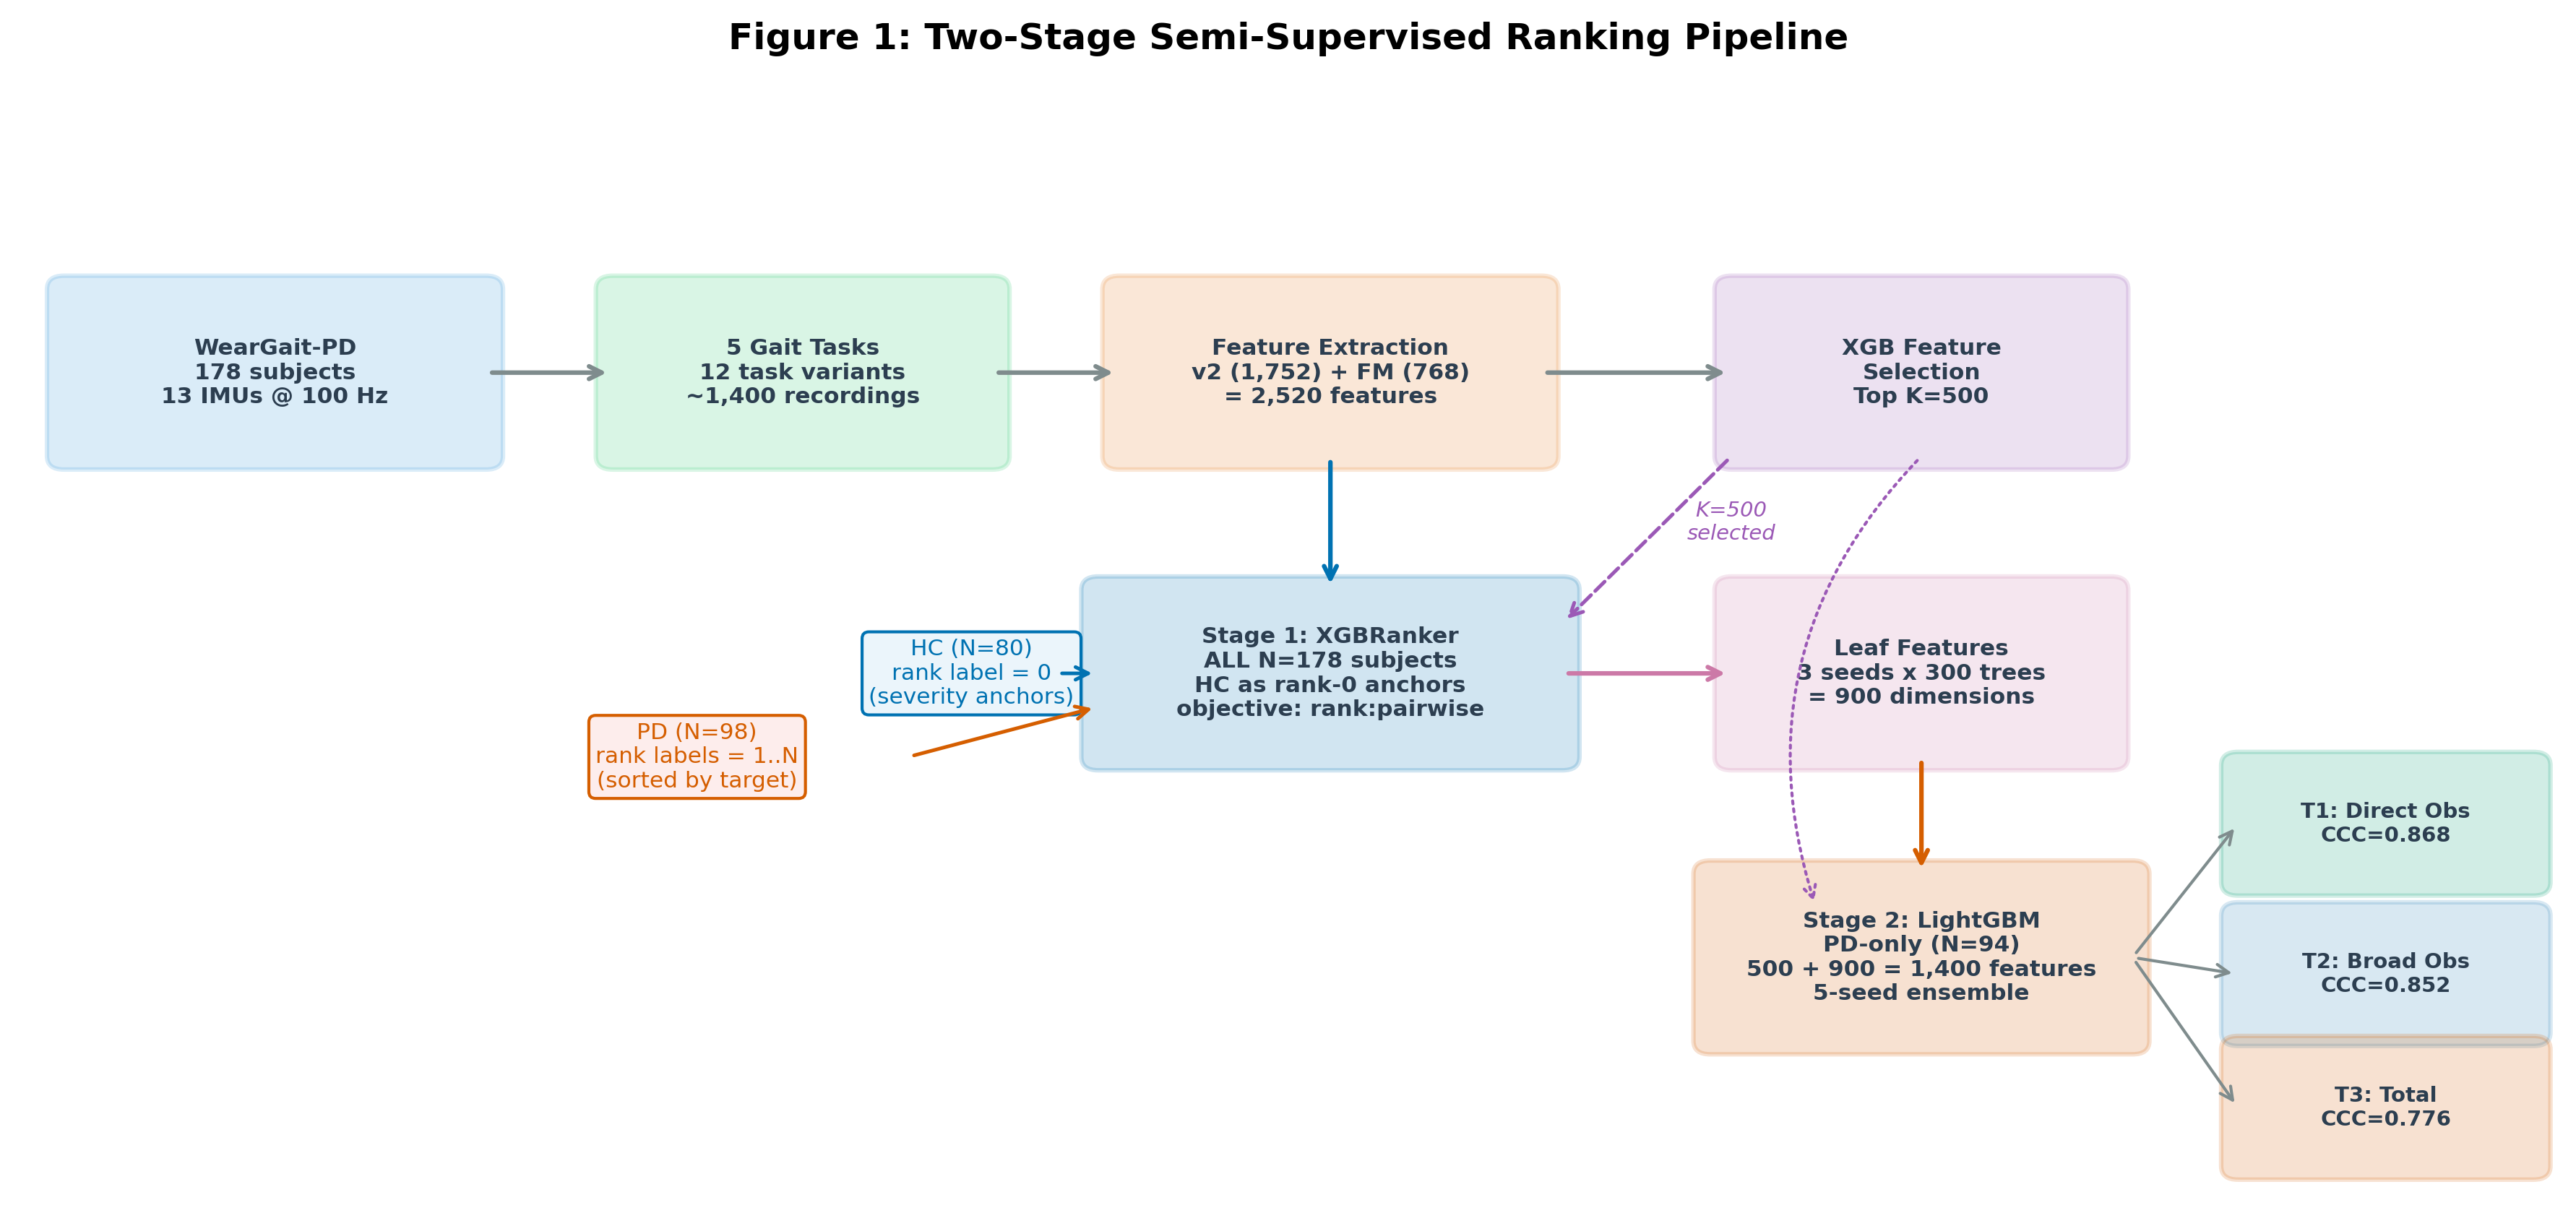
\includegraphics[width=\textwidth]{figures/fig01_pipeline.png}
\caption{Two-stage semi-supervised ranking pipeline. Stage 1: XGBRanker trained on all N=178 subjects (HC anchored at rank 0, PD subjects ranked by target score) produces leaf features encoding severity ordering. Stage 2: LightGBM regressor trained on PD-only subjects (N=94) uses original features plus 900 leaf features. Evaluated by PD-only LOOCV.}
\label{fig:pipeline}
\end{figure}

\section{Results}

\subsection{Cohort Description}

Of 185 enrolled participants, 178 (98 PD, 80 HC) had complete sensor recordings (Table~\ref{tab:demographics}). PD participants (mean age 66.9~$\pm$~8.3 years, 63M/35F) had moderate motor severity (UPDRS-III 24.4~$\pm$~10.9, range [0, 59]). HC participants were older (74.6~$\pm$~8.5 years) with lower motor scores (7.1~$\pm$~9.7). Medication state was not systematically controlled.
\begin{table}[H]
\centering
\caption{Cohort demographics.}
\label{tab:demographics}
\begin{tabular}{lll}
\toprule
Characteristic & PD (N=98) & HC (N=80) \\
\midrule
Age, years (mean $\pm$ SD) & 66.9 $\pm$ 8.3 & 74.6 $\pm$ 8.5 \\
Sex (M/F) & 63M / 35F & 35M / 45F \\
Height, cm (mean $\pm$ SD) & 174.2 $\pm$ 10.3 & 168.1 $\pm$ 17.5 \\
Weight, kg (mean $\pm$ SD) & 78.0 $\pm$ 17.2 & 81.0 $\pm$ 16.8 \\
UPDRS-III (mean $\pm$ SD) & 24.4 $\pm$ 10.9 & 7.1 $\pm$ 9.7 \\
UPDRS-III range & [0.0, 59.0] & [0.0, 43.0] \\
H\&Y (mean $\pm$ SD) & 2.15 $\pm$ 0.6 (N=95) & --- \\
H\&Y distribution & 1: 9, 1.5: 1, 2: 58, 2.5: 12, 3: 12, 4: 3 & --- \\
Years since dx (mean $\pm$ SD) & 7.6 $\pm$ 5.9 ([0.0, 26.4]) & --- \\
DBS & 23 & --- \\
\bottomrule
\end{tabular}
\end{table}

\subsection{SSL Ranking: Observable Subscore Prediction}

The directly observable subscore (items 3.9--3.14: arising, gait, freezing, postural stability, posture, body bradykinesia; max 24 points) is the primary endpoint. With SSL ranking (P5, PD-only LOOCV, N~=~94; Figure~\ref{fig:ssl_scatter}), the pipeline achieves CCC~=~0.868, calibration slope~=~0.689, MAE~=~0.986 (r~=~0.899). This represents a substantial improvement over the baseline (CCC~=~0.56, slope~=~0.401). The MAE of 0.986 falls well below the MCID of 3.25 points, indicating clinically actionable prediction accuracy.

SSL ranking also improves broader targets: T2 (items 7--14, max 32) achieves CCC~=~0.852 (MAE~=~1.33), and T3 (total UPDRS-III) achieves CCC~=~0.776 (MAE~=~4.65; Figure~\ref{fig:three_target}). The CCC degradation from T1 to T3 (0.868 to 0.776) reflects increasing inclusion of items unobservable from gait IMU.
\begin{figure}[H]
\centering
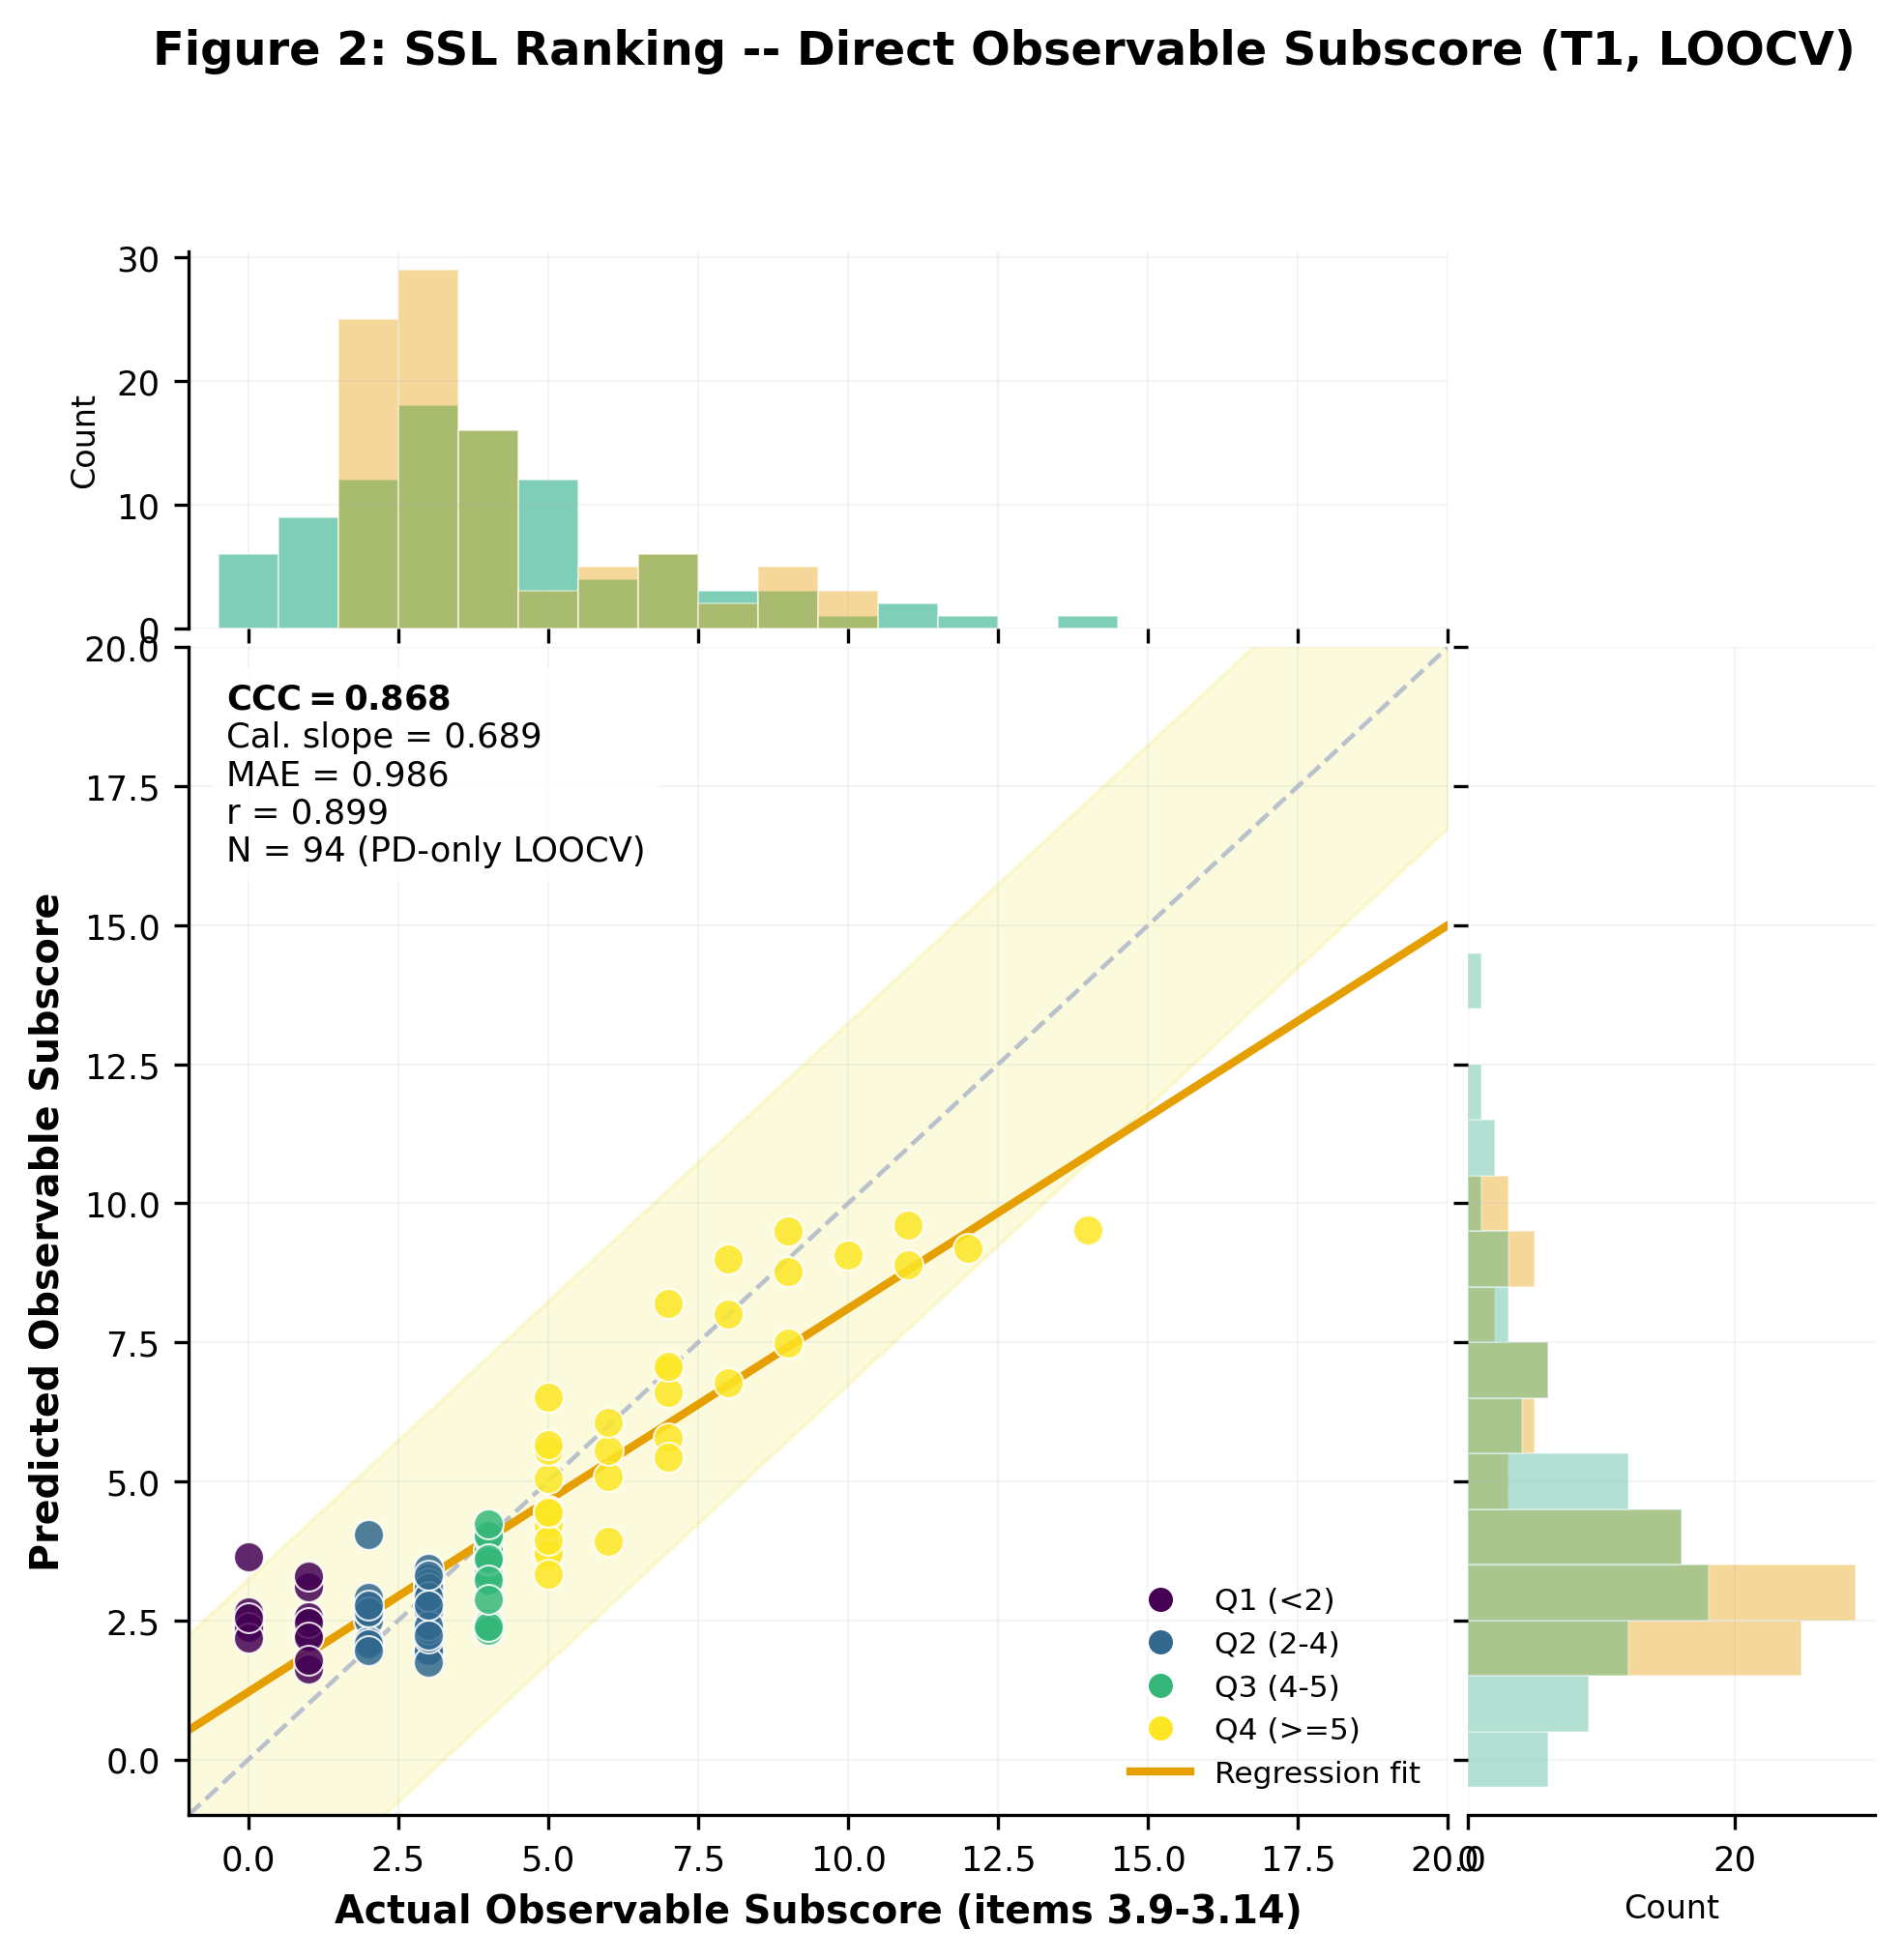
\includegraphics[width=\textwidth]{figures/fig02_ssl_scatter.png}
\caption{SSL ranking predicted versus actual scores for the directly observable subscore (T1, items 3.9--3.14), PD-only LOOCV (N=94). Points colored by severity quartile. Yellow band: $\pm$MCID (3.25). CCC~=~0.868, calibration slope~=~0.689. Marginal histograms show distribution of actual (green) and predicted (orange) scores.}
\label{fig:ssl_scatter}
\end{figure}
\begin{figure}[H]
\centering
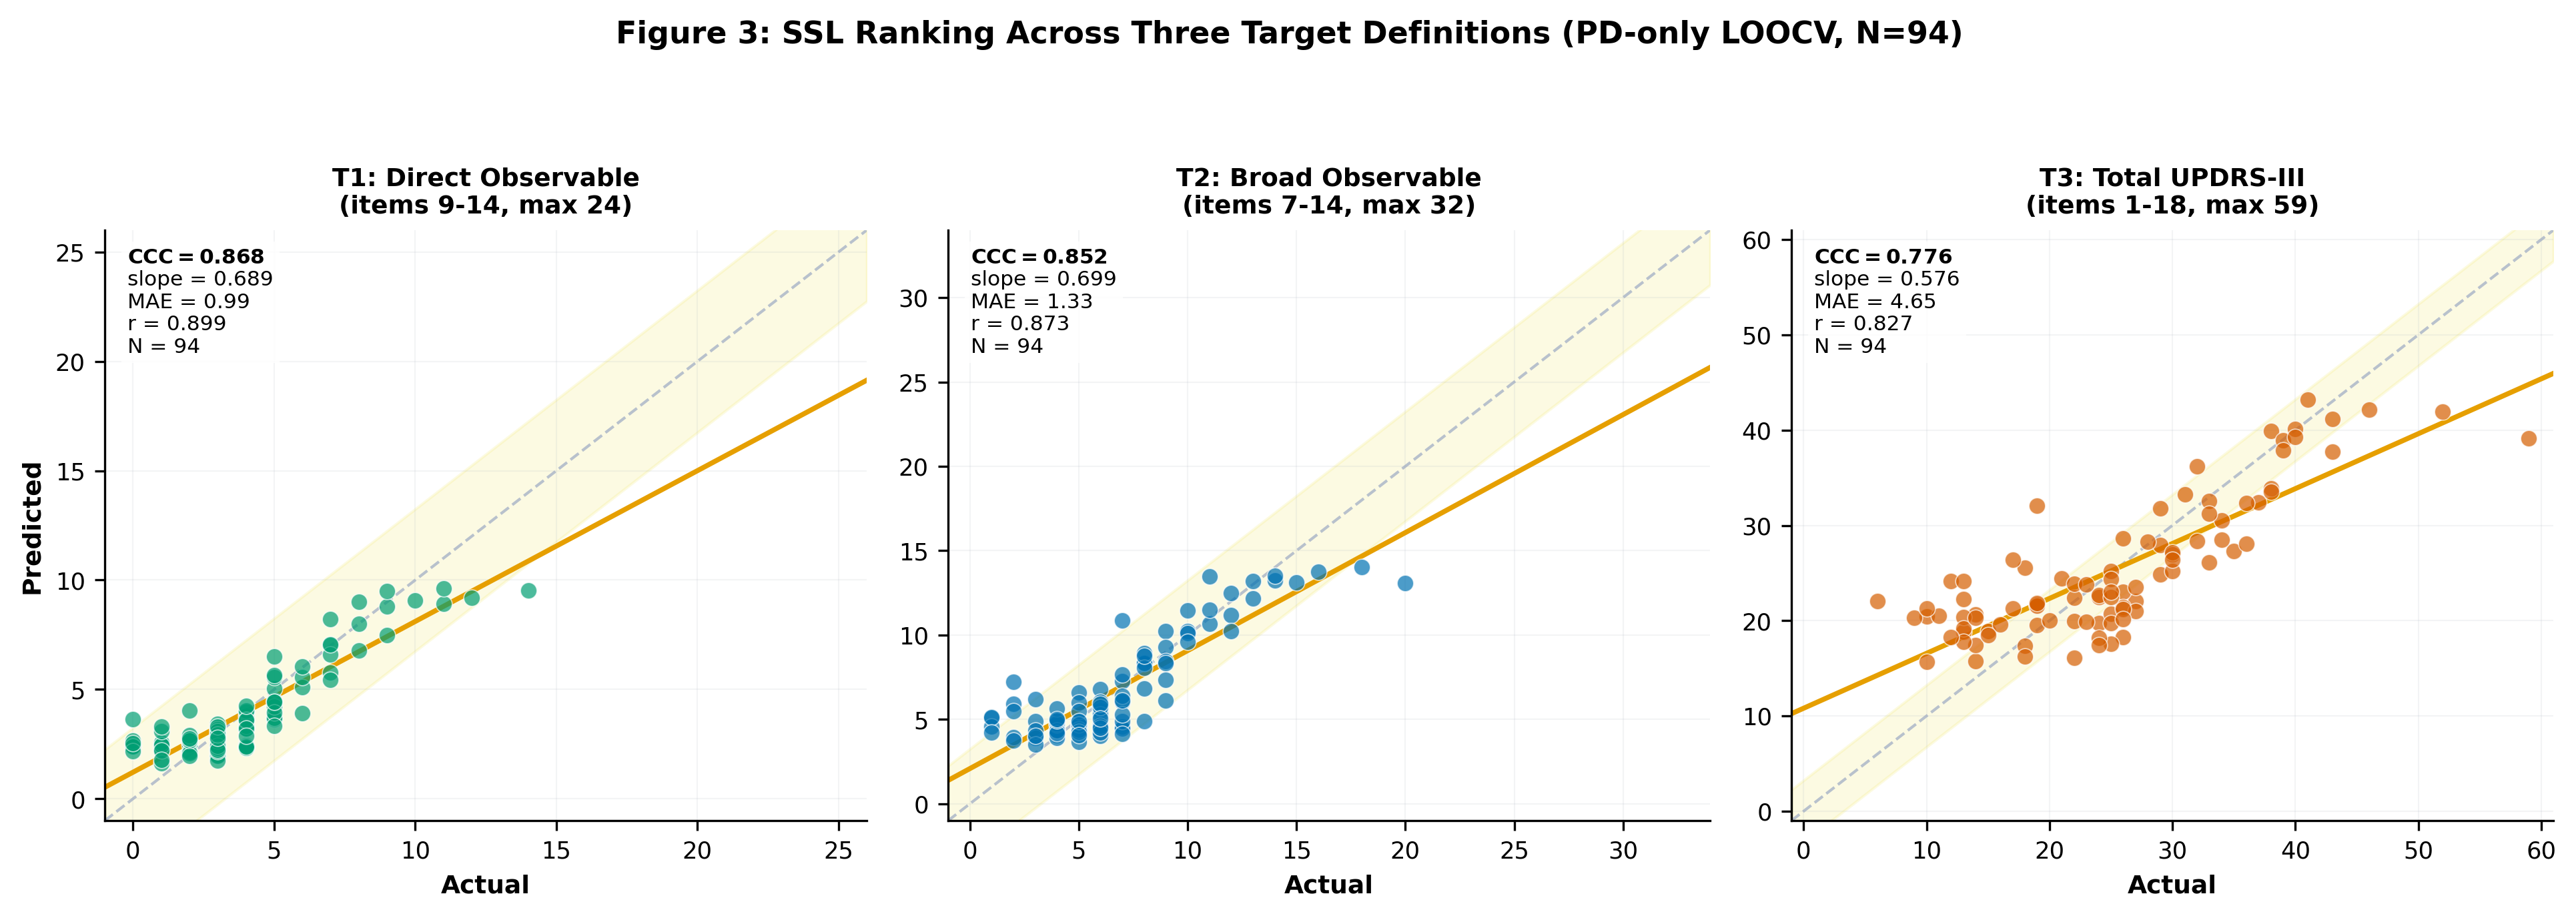
\includegraphics[width=\textwidth]{figures/fig03_three_target.png}
\caption{SSL ranking across three target definitions (PD-only LOOCV, N=94). Left: T1 direct observable (CCC=0.868). Center: T2 broad observable (CCC=0.852). Right: T3 total UPDRS-III (CCC=0.776). CCC degrades as targets include more items unobservable from gait sensors.}
\label{fig:three_target}
\end{figure}

\subsection{Three-Level Observability Decomposition}

We decomposed the 18 MDS-UPDRS-III items into three tiers based on whether the assessed motor sign is physically manifest during gait (Table~\ref{tab:observability}, Figure~\ref{fig:observability}). Using the \emph{baseline} model (pre-SSL, PD-only LOOCV), the CCC gradient is the structural finding: 0.56 (direct) vs 0.12 (partial) vs 0.18 (not observable). The partial tier (hand movements, pronation, tremor) dropped to CCC~=~0.12 (MAE~=~4.89), and the not-observable tier (speech, facial expression, rigidity) to CCC~=~0.18 (MAE~=~3.94).
\begin{figure}[H]
\centering
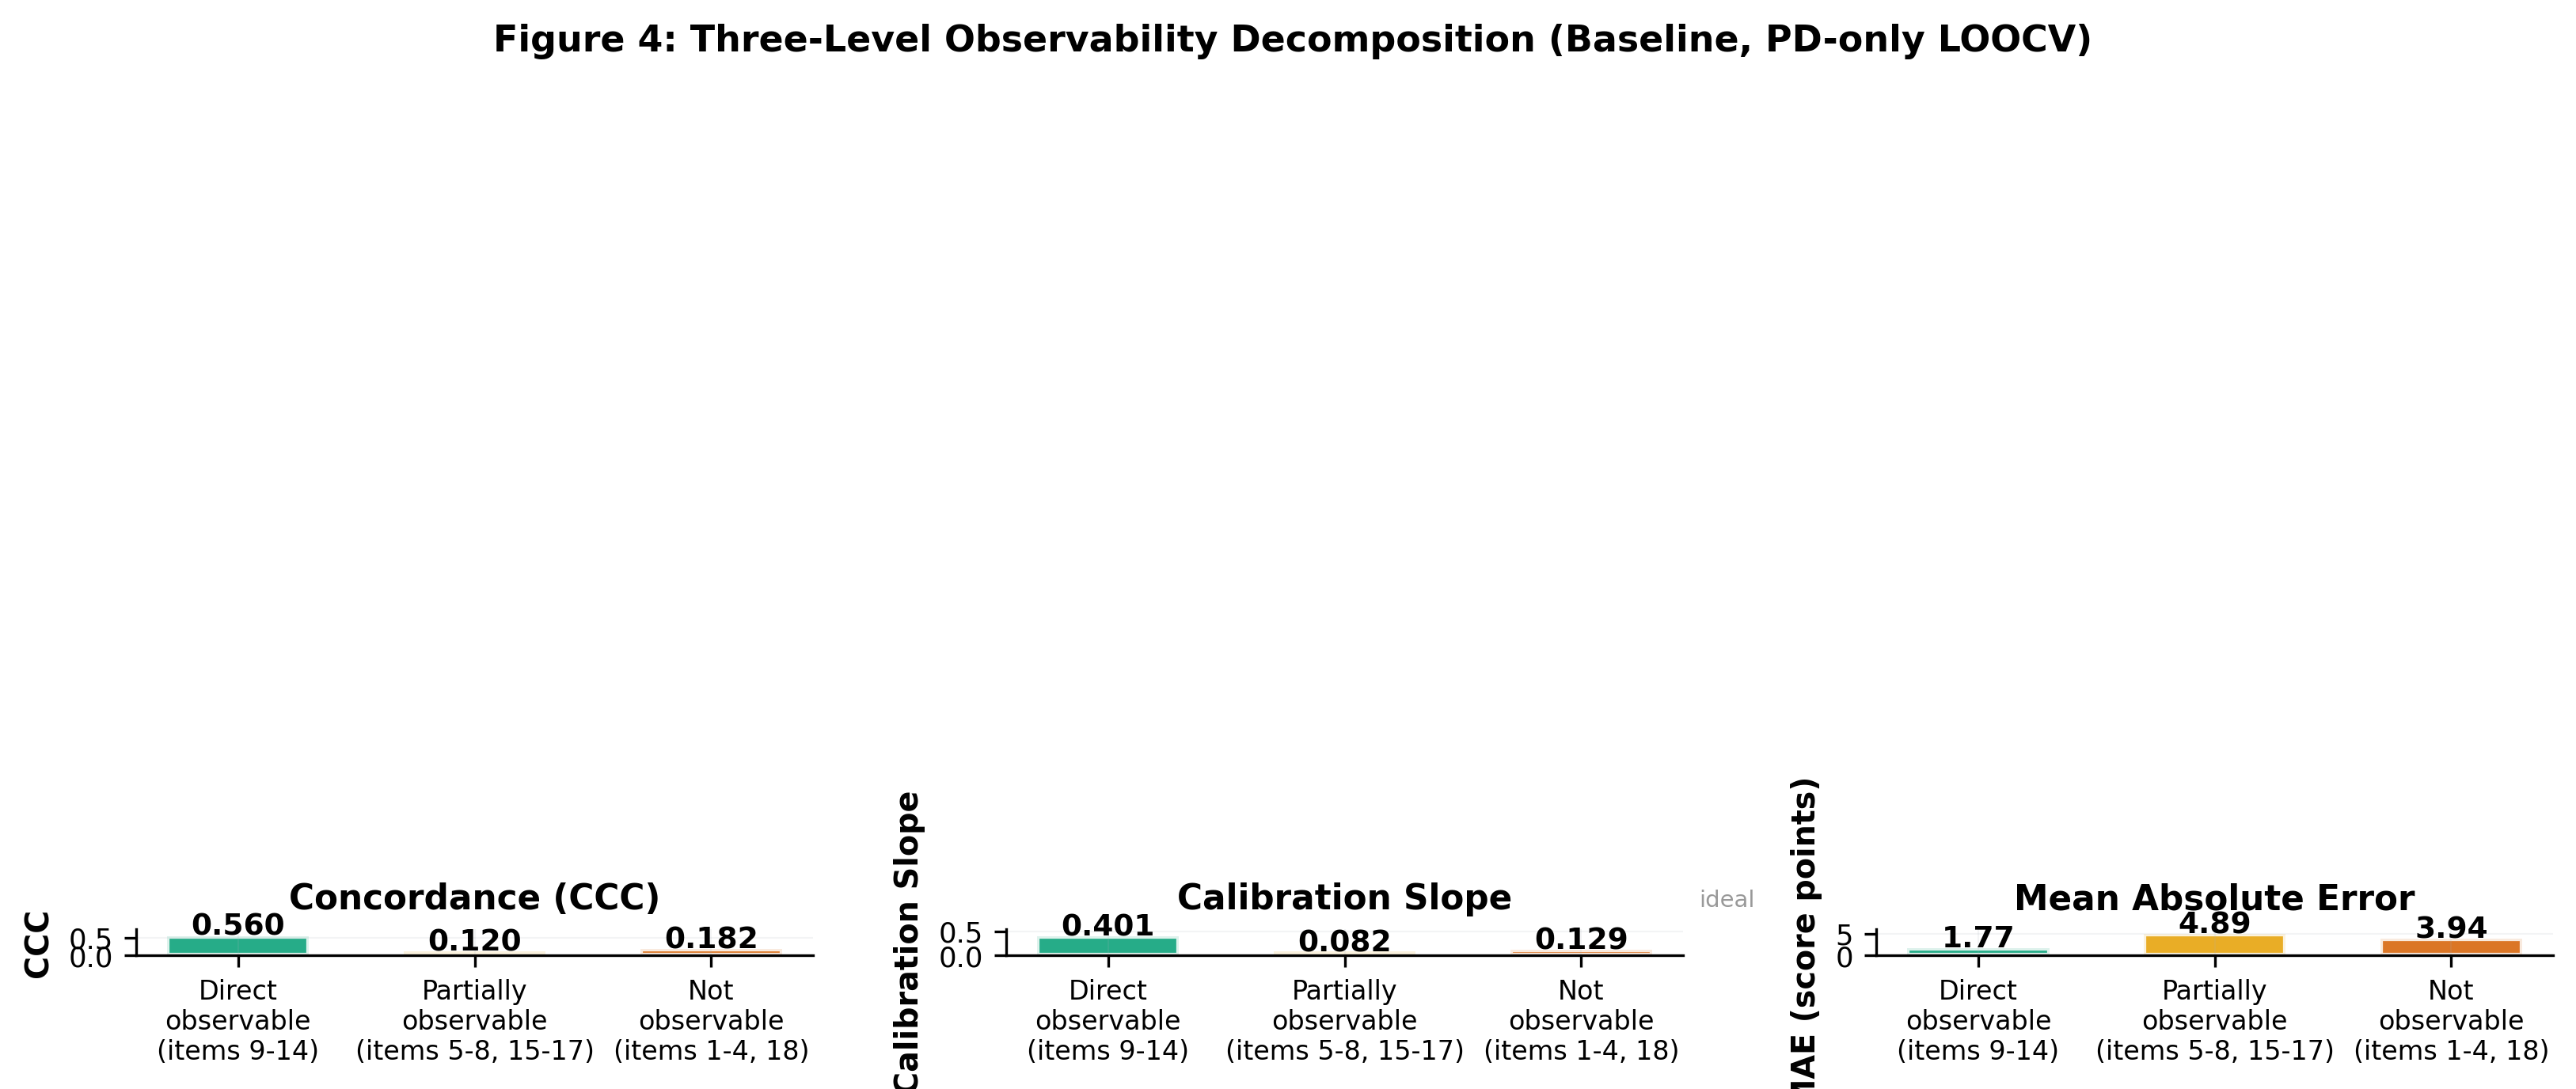
\includegraphics[width=\textwidth]{figures/fig04_observability.png}
\caption{Three-level observability decomposition (baseline model, PD-only LOOCV). CCC, calibration slope, and MAE all degrade sharply from directly observable to partially/not observable tiers. This is a modality constraint: rigidity (item 3.3), speech (3.1), and facial expression (3.2) cannot be measured by body-worn inertial sensors during gait.}
\label{fig:observability}
\end{figure}
\begin{table}[H]
\centering
\caption{Three-level observability decomposition (baseline model, PD-only LOOCV).}
\label{tab:observability}
\small
\begin{tabular}{llcccccccc}
\toprule
Tier & Items & Max & N & MAE & nMAE\% & CCC & Slope & r & 10-split MAE \\
\midrule
Directly observable & 3.9--3.14 & 24 & 94 & 1.77 & 7.4 & 0.560 & 0.401 & 0.667 & 1.72 $\pm$ 0.33 \\
Partially observable & 3.5--3.8, 3.15--3.17 & 68 & 94 & 4.89 & 7.2 & 0.120 & 0.082 & 0.169 & 3.99 $\pm$ 0.65 \\
Not observable & 3.1--3.4, 3.18 & 40 & 91 & 3.94 & 9.8 & 0.182 & 0.129 & 0.290 & 3.85 $\pm$ 0.46 \\
Binary observable & 3.7--3.14 & 40 & 94 & 3.13 & 7.8 & 0.464 & 0.315 & 0.608 & --- \\
\bottomrule
\end{tabular}

\smallskip
\footnotesize{Baseline model (pre-SSL). LOOCV: PD-only, N=91--94. nMAE = MAE / max score $\times$ 100. Direct + partial + unobs = total (reconstruction error = 0.0).}
\end{table}

\subsection{Item-Level Analysis}

Per-item analysis (Figure~\ref{fig:items}) confirms the observability gradient: the highest-correlation items are predominantly directly observable gait items. Feature importance for the observable subscore (Figure~\ref{fig:features}) shows clinically coherent sensor-item alignment: foot sensors (R\_DorsalFoot), lower back, and trunk (Xiphoid) drive predictions, while foundation model embedding dimensions provide complementary temporal patterns.
\begin{figure}[H]
\centering
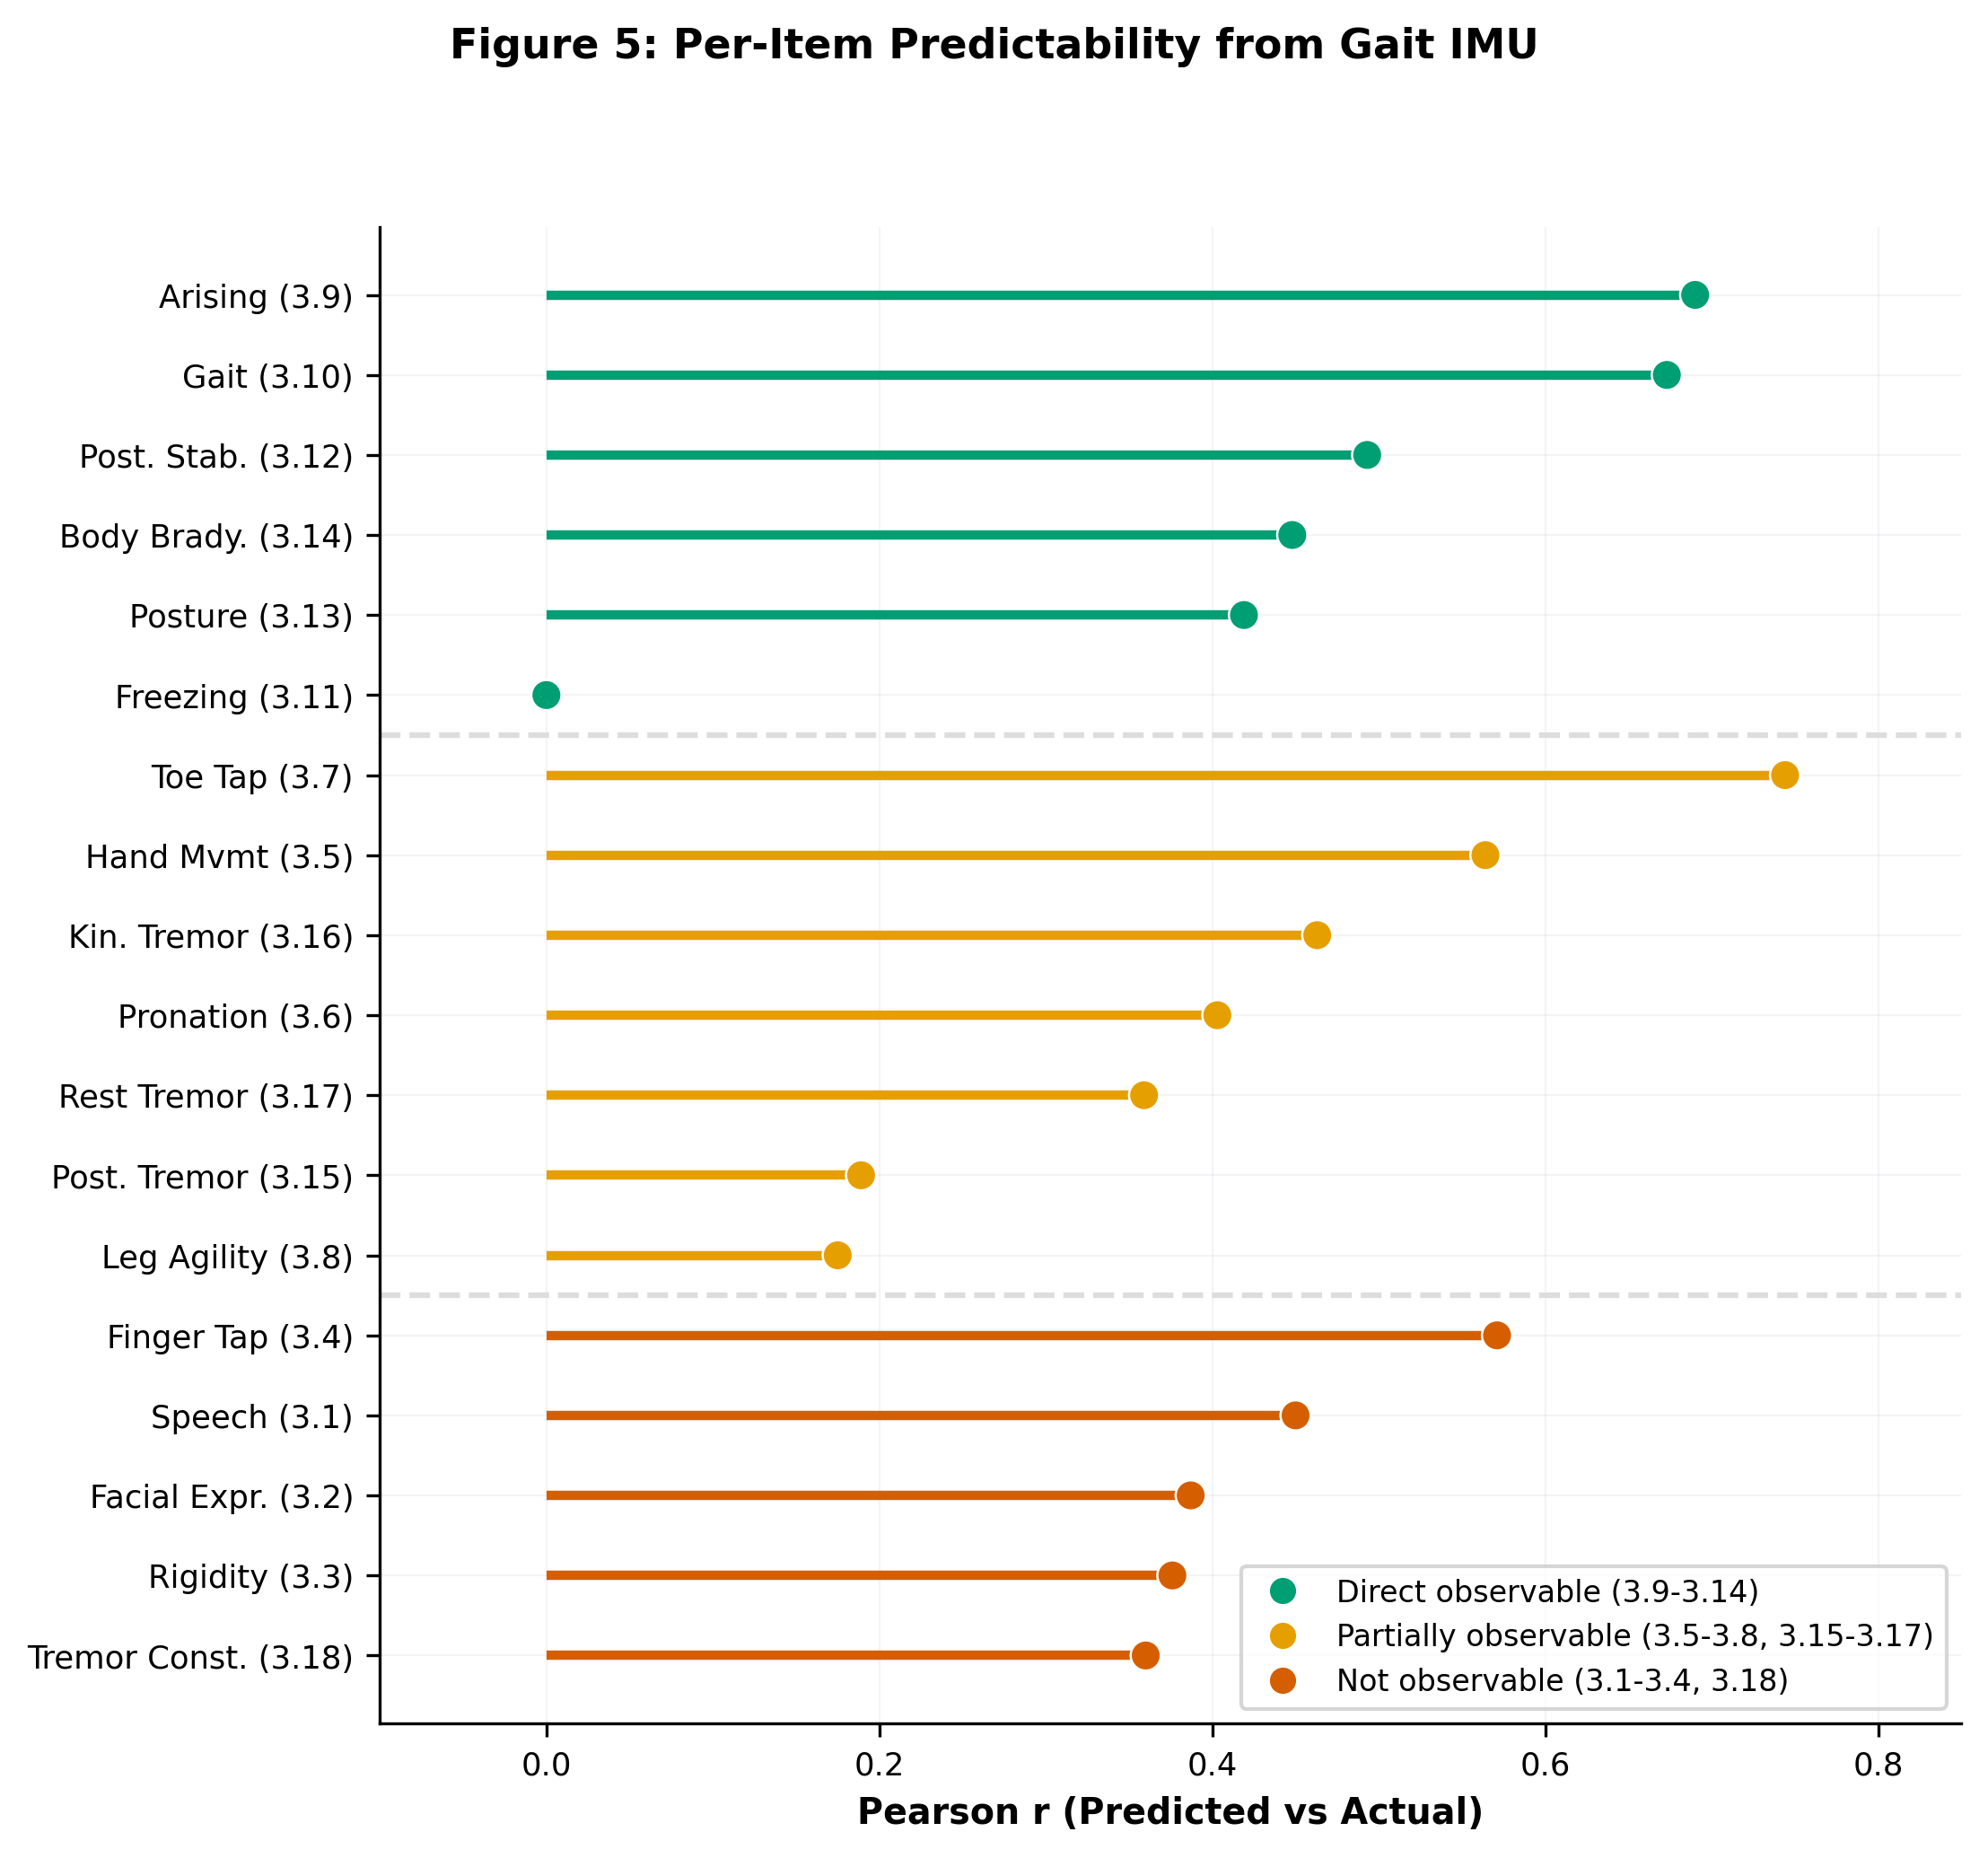
\includegraphics[width=\textwidth]{figures/fig05_item_predictability.png}
\caption{Per-item predictability ranked by Pearson r, colored by three-level observability tier. Green: directly observable from gait; orange: partially observable; red: not observable. Dashed lines separate tiers.}
\label{fig:items}
\end{figure}
\begin{figure}[H]
\centering
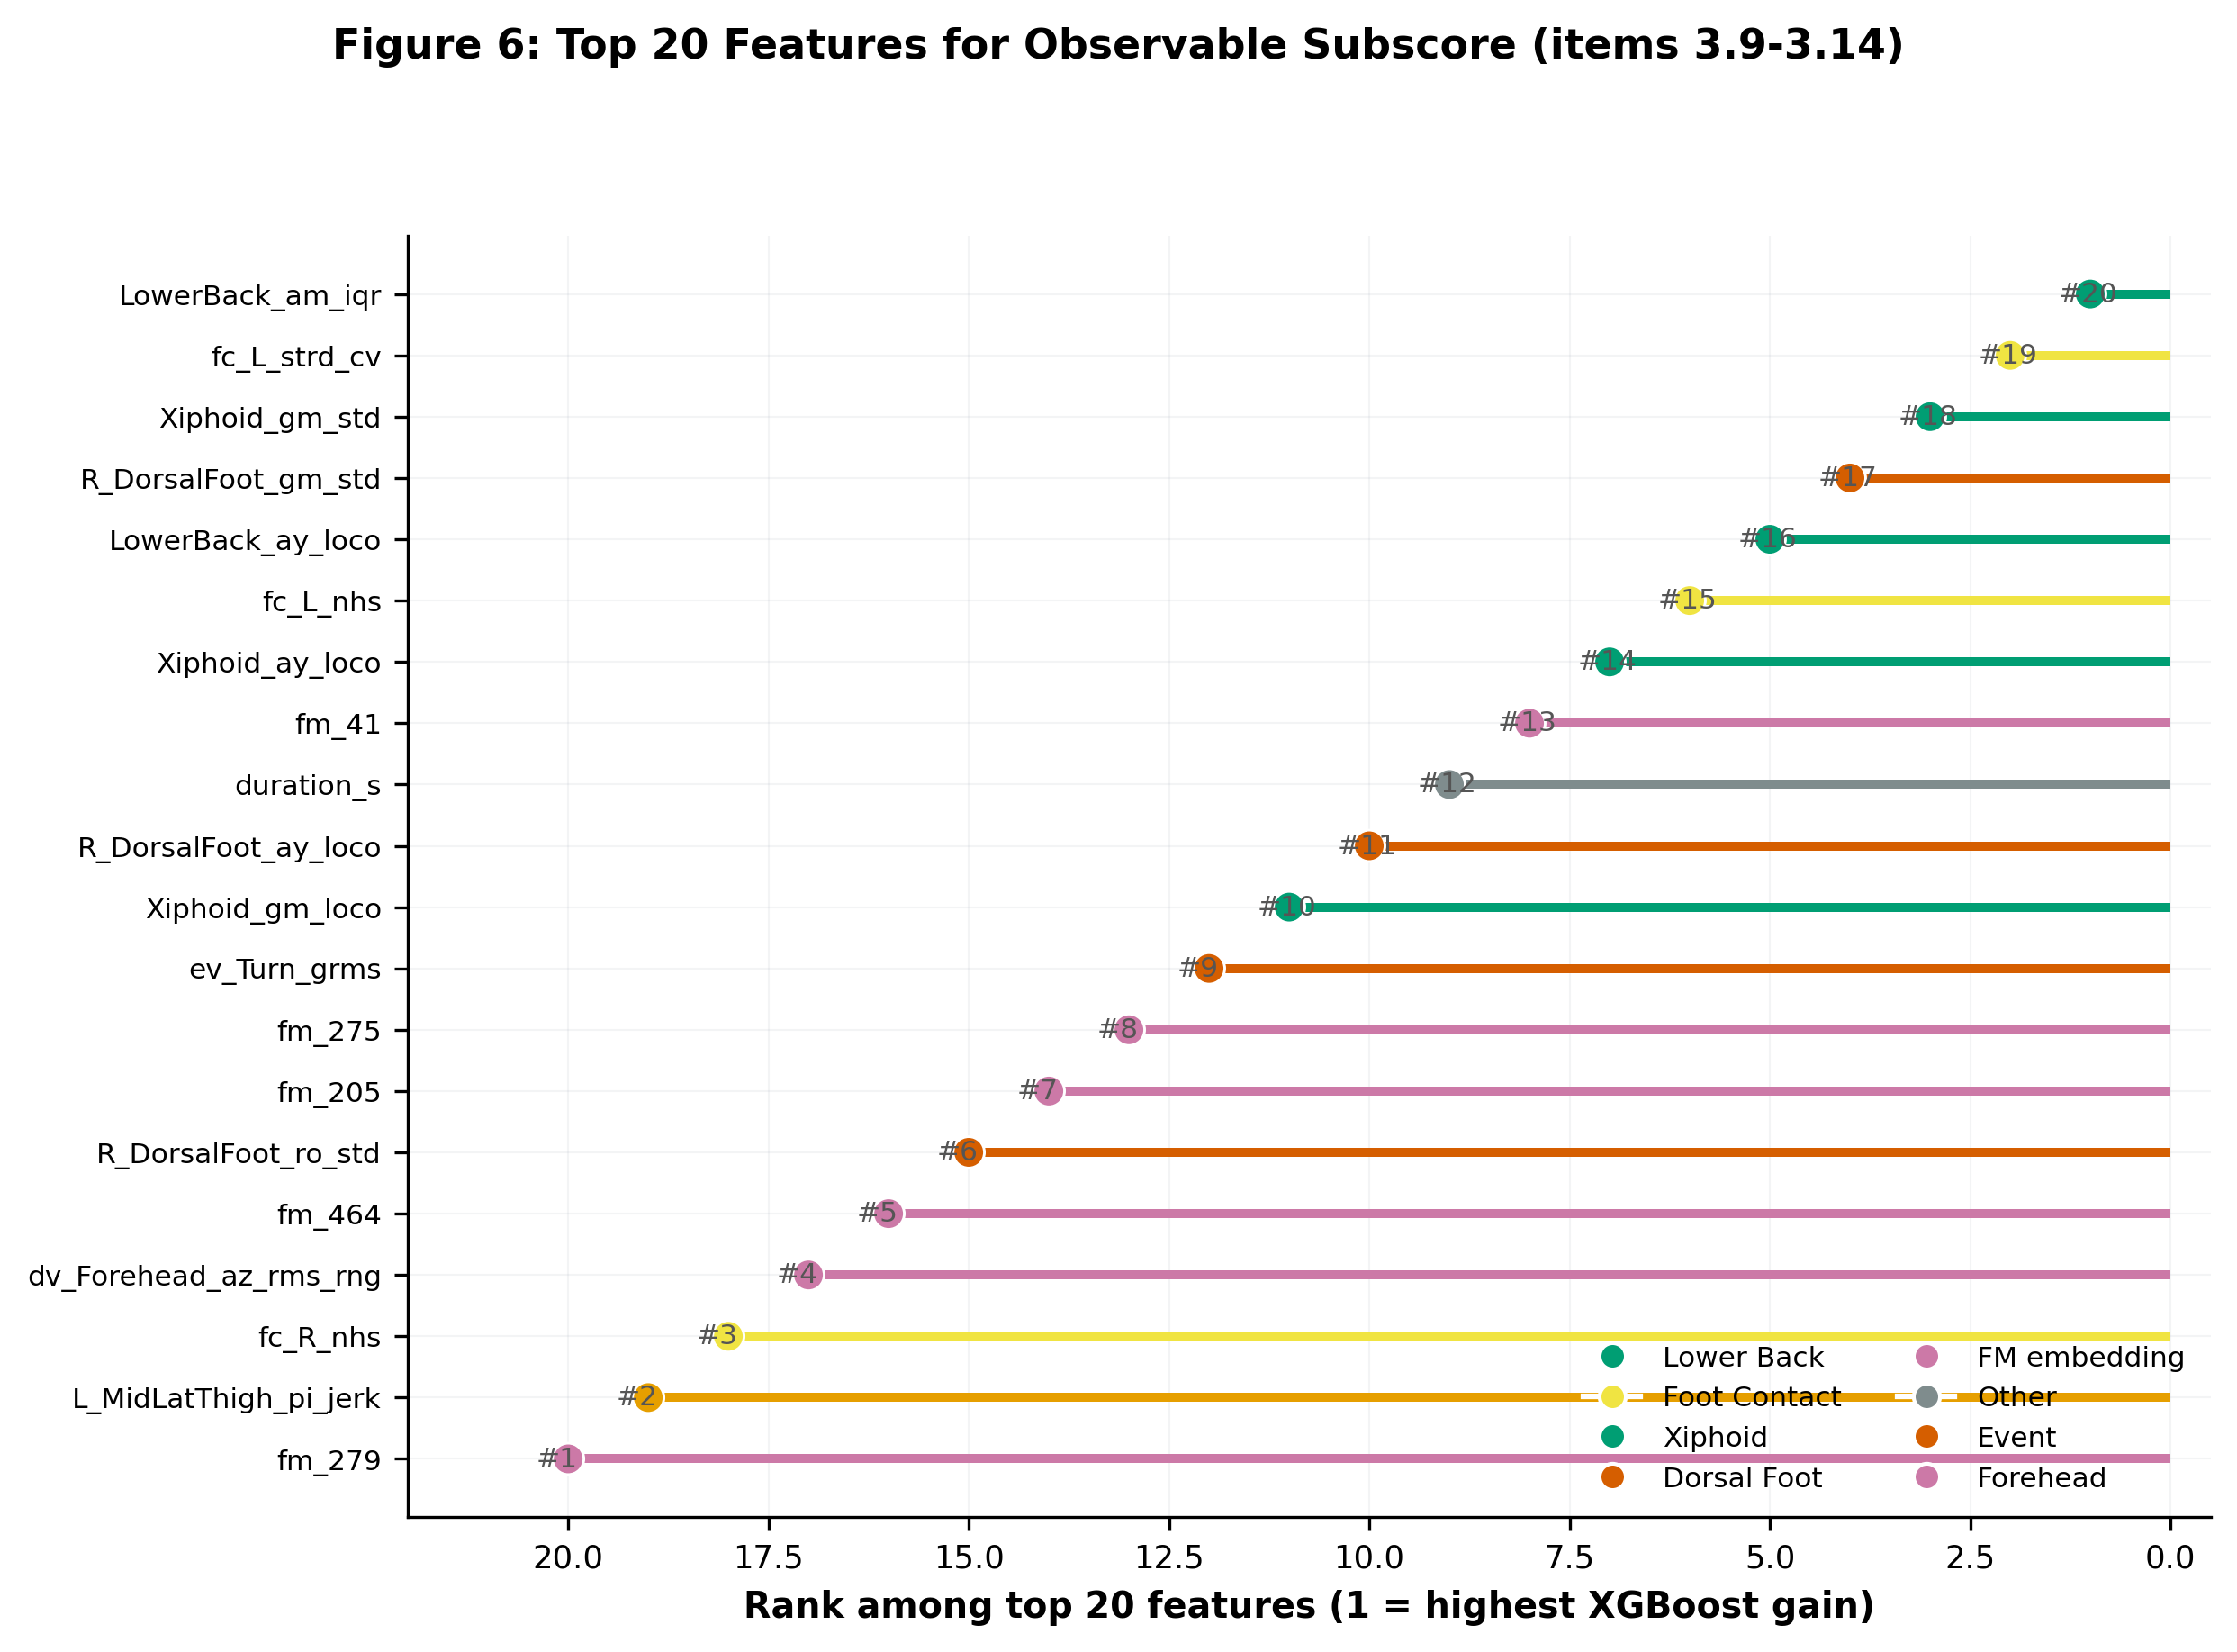
\includegraphics[width=\textwidth]{figures/fig06_feature_importance.png}
\caption{Top 20 features by XGBoost gain importance for the observable subscore model, colored by anatomical source. Foot and trunk sensors dominate, with FM embedding dimensions (fm\_*) providing complementary temporal features.}
\label{fig:features}
\end{figure}

\subsection{Compression Ablation: Why SSL Ranking Works}

We evaluated five anti-compression proposals across three targets (Table~\ref{tab:ssl_ablation}, Figure~\ref{fig:compression}). Per-item ordinal classification (P1) degraded performance severely (CCC~=~0.338). SMOGN tail augmentation (P3) and NGBoost distributional regression (P4) produced marginal improvements. Only SSL ranking (P5) materially improved CCC on all targets. The mechanism involves four elements: (i) N amplification (N=94 PD to N=178 for ranking), (ii) HC subjects as rank-0 calibration anchors, (iii) ranking as a simpler task than regression, and (iv) leaf features as nonlinear severity embeddings.
\begin{figure}[H]
\centering
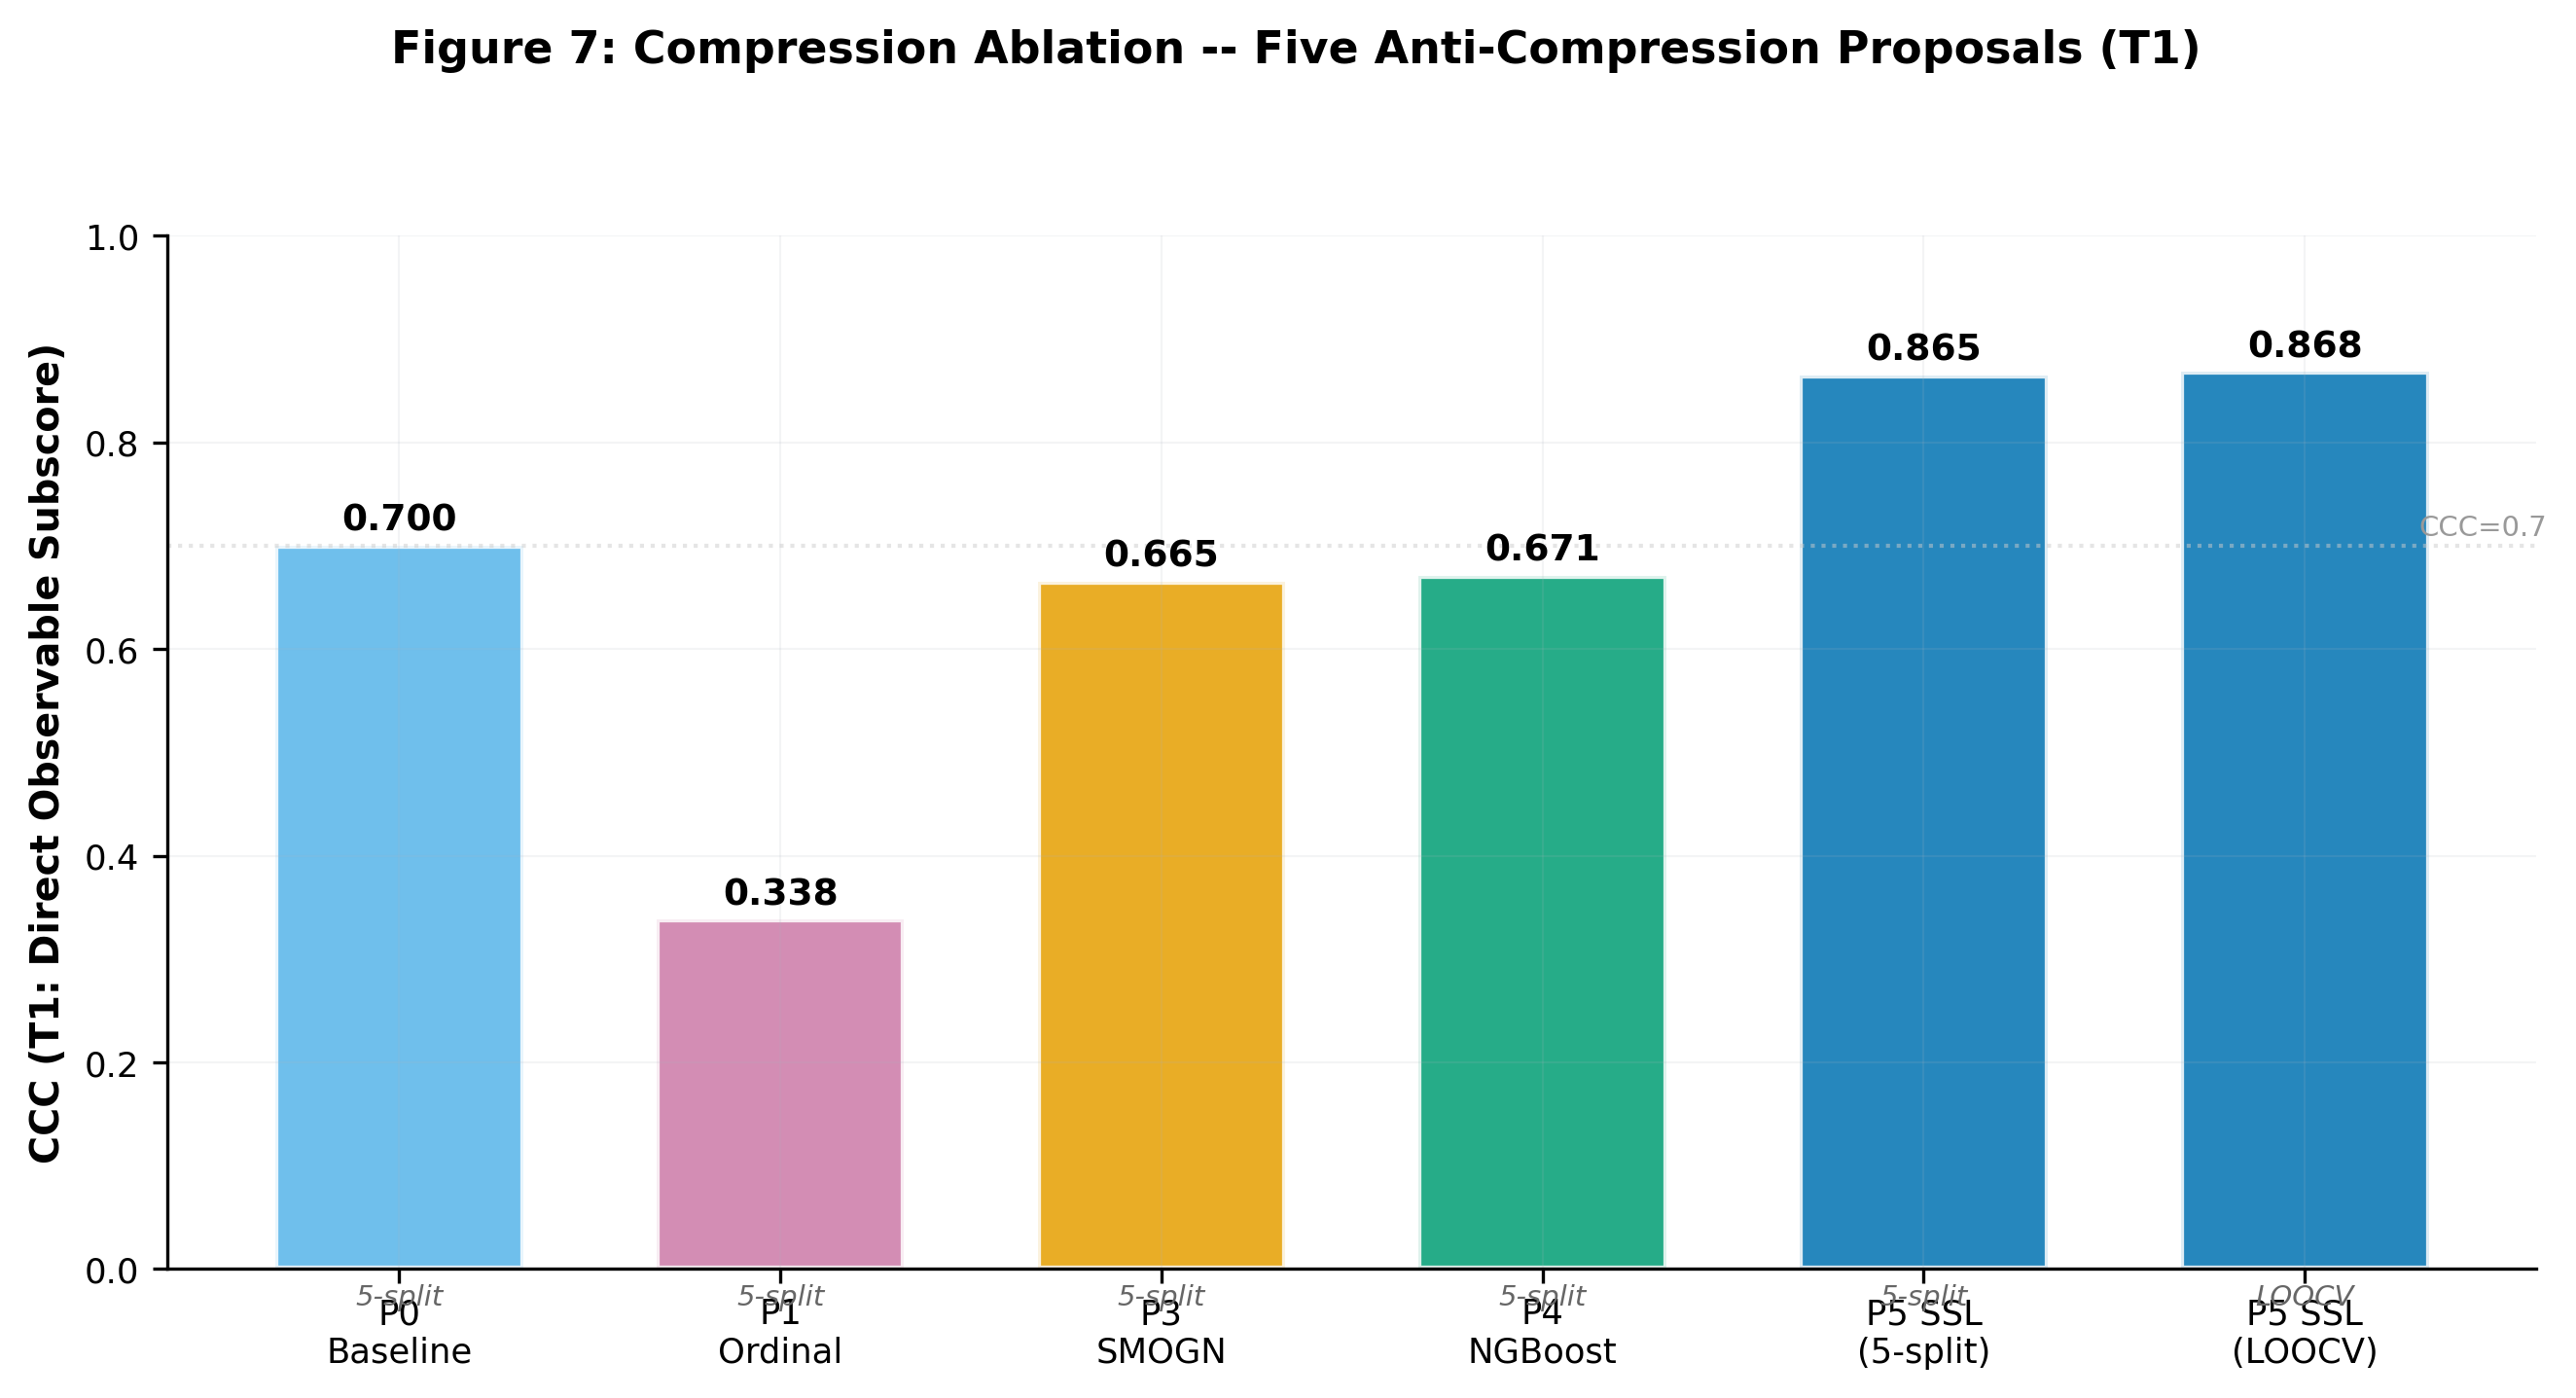
\includegraphics[width=\textwidth]{figures/fig07_compression_ablation.png}
\caption{Compression ablation: five proposals evaluated on T1 (direct observable subscore). Only P5 SSL ranking materially improves CCC. P1 ordinal classification degrades performance severely. Note: P0--P4 use 5-split evaluation; P5 (LOOCV) shown alongside for reference.}
\label{fig:compression}
\end{figure}
\begin{table}[H]
\centering
\caption{Compression ablation: five anti-compression proposals across three targets.}
\label{tab:ssl_ablation}
\small
\begin{tabular}{llccccccccc}
\toprule
 & & & \multicolumn{3}{c}{T1 (Direct Obs)} & \multicolumn{2}{c}{T2 (Broad Obs)} & \multicolumn{2}{c}{T3 (Total)} \\
\cmidrule(lr){4-6} \cmidrule(lr){7-8} \cmidrule(lr){9-10}
Proposal & Eval & N & CCC & Slope & MAE & CCC & MAE & CCC & MAE \\
\midrule
P0 Baseline & 5-split & 95 & 0.700 & 0.508 & 1.336 & 0.554 & 1.85 & 0.186 & 8.09 \\
P1 Ordinal & 5-split & 95 & 0.338 & 0.184 & 1.594 & --- & --- & --- & --- \\
P3 SMOGN & 5-split & 95 & 0.665 & 0.528 & 1.491 & 0.603 & 1.85 & 0.195 & 8.38 \\
P4 NGBoost & 5-split & 95 & 0.671 & 0.484 & 1.387 & 0.595 & 1.75 & 0.187 & 8.20 \\
\textbf{P5 SSL Ranking} & \textbf{5-split} & \textbf{95} & \textbf{0.865} & \textbf{0.745} & \textbf{0.953} & \textbf{0.831} & \textbf{1.16} & \textbf{0.807} & \textbf{4.46} \\
\textbf{P5 SSL Ranking} & \textbf{LOOCV} & \textbf{94} & \textbf{0.868} & \textbf{0.689} & \textbf{0.986} & \textbf{0.852} & \textbf{1.33} & \textbf{0.776} & \textbf{4.65} \\
\bottomrule
\end{tabular}

\smallskip
\footnotesize{P0--P4: 5-split (N=95). P5 SSL shown under both 5-split (N=95, protocol-matched with P0--P4) and LOOCV (N=94, strictest evaluation). P1 not run on T2/T3 (severely degraded on T1). P5 is the only proposal that materially improves CCC on any target.}
\end{table}

\subsection{Quartile Bias Reduction}

SSL ranking substantially reduces severity-dependent prediction bias (Table~\ref{tab:quartile_bias}, Figure~\ref{fig:quartile}). For T1 (5-split, apples-to-apples comparison): Q4 underprediction reduced from $-$1.34 to $-$0.53 (61\% reduction), Q2 overprediction nearly eliminated (from +0.67 to +0.13, 81\% reduction). The total UPDRS baseline showed extreme compression: Q1 overpredicted by +14 points, Q4 underpredicted by $-$14 points (Table~\ref{tab:severity}). After SSL ranking, T3 Q4 bias reduced from $-$12.3 to $-$3.7.
\begin{figure}[H]
\centering
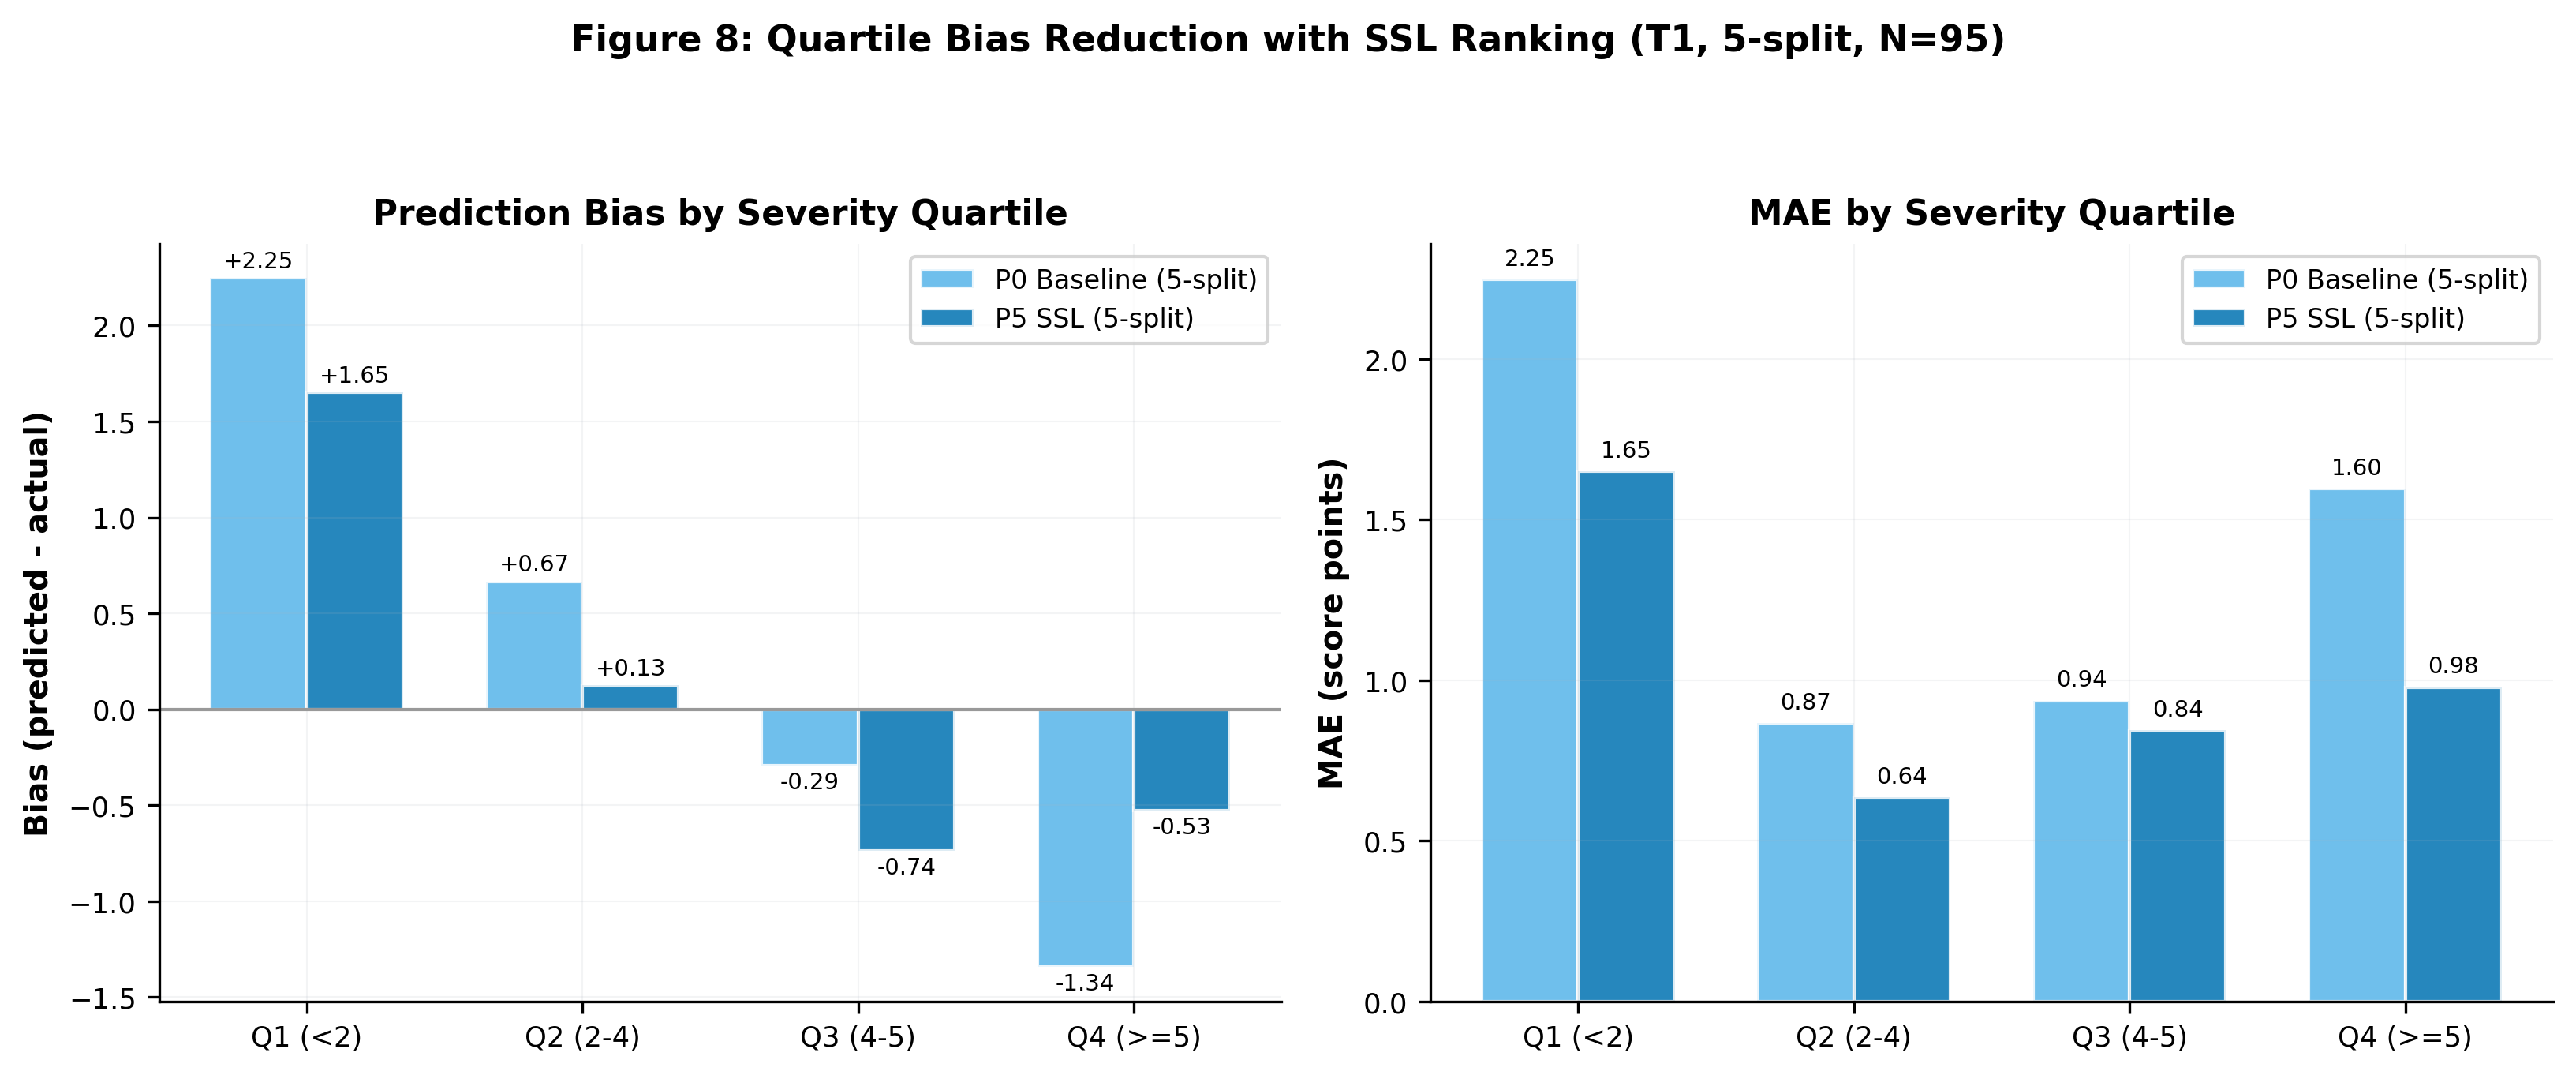
\includegraphics[width=\textwidth]{figures/fig08_quartile_bias.png}
\caption{Quartile bias reduction with SSL ranking (T1, 5-split comparison, N=95). Left: prediction bias by severity quartile. Right: MAE by quartile. SSL ranking (blue) reduces both bias and error across most quartiles compared to baseline (light blue).}
\label{fig:quartile}
\end{figure}
\begin{table}[H]
\centering
\caption{Quartile bias analysis: P0 baseline vs P5 SSL (both 5-split, N=95), T1 direct observable.}
\label{tab:quartile_bias}
\small
\begin{tabular}{lccccccl}
\toprule
 & \multicolumn{3}{c}{P0 Baseline (5-split)} & \multicolumn{3}{c}{P5 SSL (5-split)} & \\
\cmidrule(lr){2-4} \cmidrule(lr){5-7}
Quartile & N & Bias & MAE & N & Bias & MAE & $|$Bias$|$ Change \\
\midrule
Q1 (<2) & 16 & +2.25 & 2.25 & 16 & +1.65 & 1.65 & -27\% \\
Q2 (2-4) & 31 & +0.67 & 0.87 & 31 & +0.13 & 0.64 & -81\% \\
Q3 (4-5) & 19 & -0.29 & 0.94 & 19 & -0.74 & 0.84 & +151\% \\
Q4 (>=5) & 29 & -1.34 & 1.60 & 29 & -0.53 & 0.98 & -61\% \\
\bottomrule
\end{tabular}

\smallskip
\footnotesize{Both P0 and P5 use identical 5-split evaluation protocol (N=95) for apples-to-apples comparison. Bias = mean(predicted $-$ actual).}
\end{table}

\subsection{Total UPDRS-III as Context}

Total UPDRS-III prediction illustrates the structural ceiling that motivates the observable subdomain focus. In PD-only 10-split CV (N~=~98, Table~\ref{tab:total_updrs}), a demographic Ridge baseline (age, sex, disease duration) achieved MAE~=~7.44~$\pm$~0.75, matching all IMU models. Partial correlation r~=~0.36 (p$_{\text{adj}}$~=~0.002) confirms genuine IMU signal beyond demographics, but this signal is diluted by 12 partially or non-observable items constituting 82\% of the total score range. After SSL ranking, IMU clearly surpasses demographics: T3 MAE~=~4.65 vs demographic MAE~=~7.86.
\begin{table}[H]
\centering
\caption{Total UPDRS-III prediction results (PD-only evaluation).}
\label{tab:total_updrs}
\begin{tabular}{llccccc}
\toprule
Model & Evaluation & N & MAE & CCC & r & Cal.\ slope \\
\midrule
\multicolumn{7}{l}{\textit{PD-only 10-split cross-validation}} \\
Demographic Ridge & 10-split & 98 & 7.44 $\pm$ 0.75 & 0.326 & --- & --- \\
v2 Handcrafted LGB & 10-split & 98 & 8.42 $\pm$ 0.69 & -0.004 & --- & --- \\
v2+FM Stack & 10-split & 98 & 8.57 $\pm$ 0.96 & -0.019 & --- & --- \\
\midrule
\multicolumn{7}{l}{\textit{PD-only leave-one-out cross-validation}} \\
FM Stack (baseline) & LOOCV & 98 & 8.15 & 0.369 & 0.429 & 0.256 \\
Demographic Ridge & LOOCV & 98 & 7.86 & 0.338 & 0.427 & 0.211 \\
\midrule
\multicolumn{7}{l}{\textit{Anti-compression methods (PD-only)}} \\
P0 Baseline & 5-split & 95 & 8.09 & 0.186 & 0.297 & 0.104 \\
\textbf{P5 SSL Ranking} & \textbf{LOOCV} & \textbf{94} & \textbf{4.65} & \textbf{0.776} & \textbf{0.827} & \textbf{0.576} \\
\bottomrule
\end{tabular}

\smallskip
\footnotesize{P0 baseline and P5 SSL use different evaluation protocols (5-split vs LOOCV). P5 SSL uses healthy controls for representation learning only; final evaluation is PD-only.}
\end{table}
\begin{table}[H]
\centering
\caption{Severity-stratified prediction (baseline, PD-only FM LOOCV, N=98).}
\label{tab:severity}
\begin{tabular}{lcccccc}
\toprule
Quartile & N & MAE & CCC & Bias & Mean True & Mean Pred \\
\midrule
Q1(<12) & 9 & 14.09 & 0.141 & +14.1 & 6.2 & 20.3 \\
Q2(12-20) & 26 & 5.96 & 0.068 & +4.5 & 15.6 & 20.1 \\
Q3(20-35) & 46 & 5.94 & 0.152 & -4.0 & 26.8 & 22.7 \\
Q4(>35) & 17 & 14.30 & 0.138 & -14.3 & 41.2 & 26.9 \\
\bottomrule
\end{tabular}

\smallskip
\footnotesize{Bias = mean(predicted $-$ actual). Severe regression to the mean: Q1 overpredicted by +14, Q4 underpredicted by $-$14. Pre-SSL baseline.}
\end{table}

\subsection{Foundation Model Impact}

Frozen MOMENT-1-base embeddings (768 dimensions, no fine-tuning) reduced mixed-cohort MAE from 8.49 to 7.77 (Wilcoxon p~=~0.0039; Figure~\ref{fig:fm}). The advantage was non-significant in PD-only evaluation (p$_{\text{adj}}$~=~0.94), suggesting FM embeddings primarily enhance PD-vs-HC discrimination rather than within-PD severity grading. FM embedding dimensions appeared among top features for the observable subscore (Figure~\ref{fig:features}), indicating complementary temporal pattern capture beyond handcrafted statistics.
\begin{figure}[H]
\centering
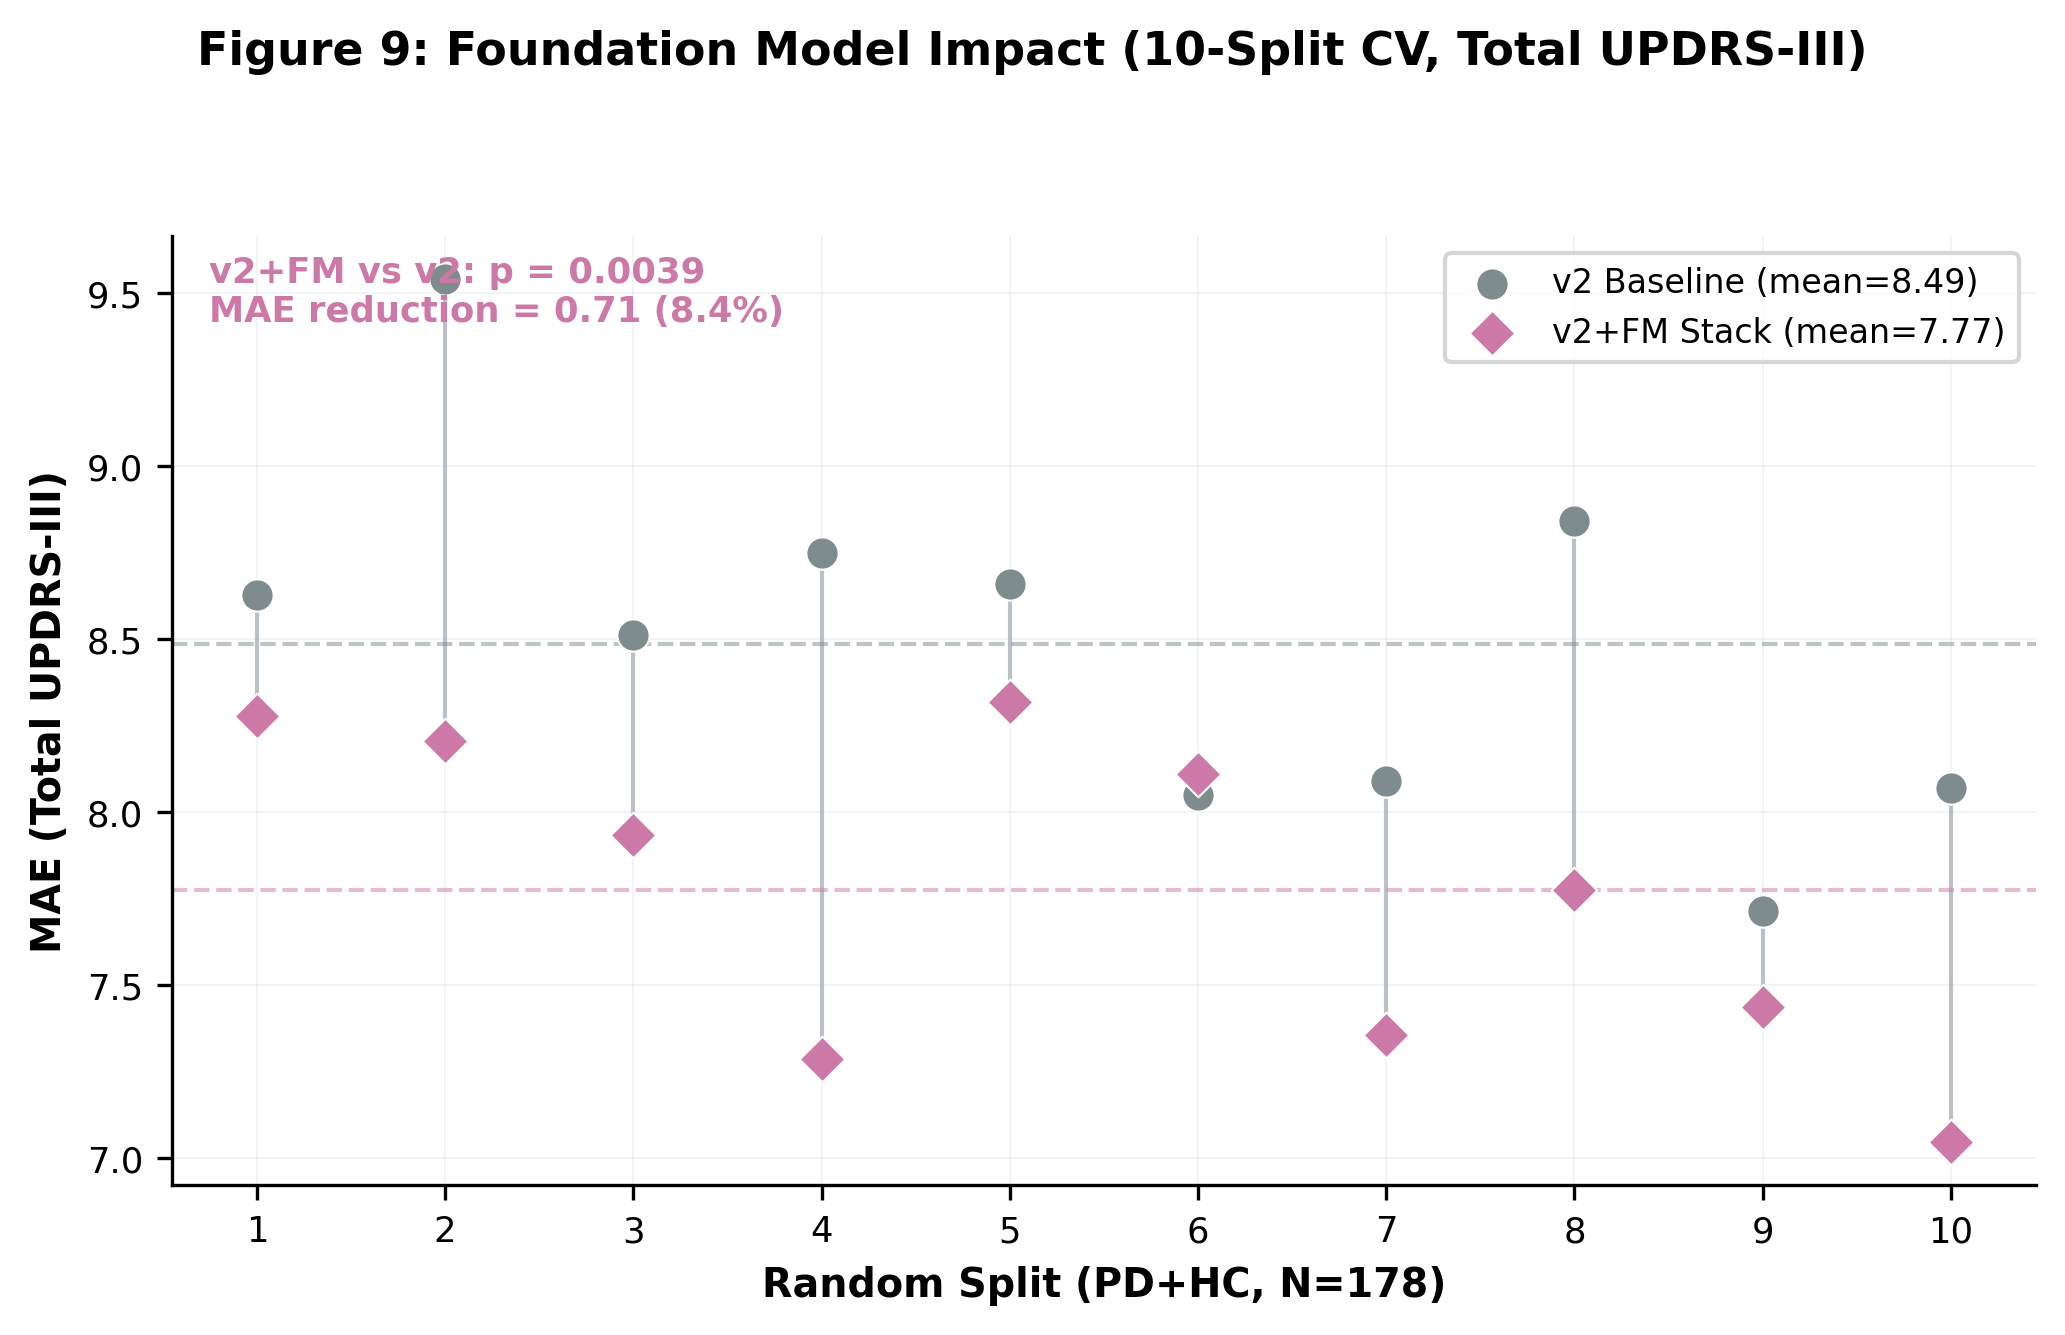
\includegraphics[width=\textwidth]{figures/fig09_fm_impact.png}
\caption{Foundation model impact across 10 splits (PD+HC, N=178, total UPDRS-III). v2+FM stack (purple diamonds) consistently outperforms v2 baseline (grey circles). Paired Wilcoxon p~=~0.0039.}
\label{fig:fm}
\end{figure}

\subsection{Sensor Ablation}

FM re-extraction per sensor configuration eliminates data leakage (Table~\ref{tab:sensor}). The 5-sensor minimal set (lower back, bilateral wrists, bilateral ankles) matches the full 13-sensor configuration (7.67 vs 7.72, p~=~0.85). Even 2 wrist sensors achieved competitive performance (p~=~0.55). These results are for total UPDRS-III; observable-subscore sensor ablation has not been conducted.
\begin{table}[H]
\centering
\caption{Sensor ablation (PD-only 10-split, total UPDRS-III, FM re-extracted per config).}
\label{tab:sensor}
\begin{tabular}{lcccl}
\toprule
Configuration & N Sensors & MAE $\pm$ SD & CCC & p vs All 13 \\
\midrule
All 13 sensors & 13 & 7.72 $\pm$ 0.78 & 0.184 & --- \\
Minimal 5 (back+wrists+ankles) & 5 & 7.67 $\pm$ 0.84 & 0.152 & 0.851 \\
Back + wrists (3) & 3 & 7.89 $\pm$ 0.64 & 0.113 & 0.202 \\
Wrists only (2) & 2 & 7.80 $\pm$ 0.63 & 0.102 & 0.555 \\
Lower back only (1) & 1 & 8.12 $\pm$ 0.76 & 0.048 & 0.014 \\
\bottomrule
\end{tabular}

\smallskip
\footnotesize{FM embeddings re-extracted per sensor configuration to prevent data leakage. Results are for total UPDRS-III, not observable subscore.}
\end{table}

\subsection{Cross-Dataset Context}

Figure~\ref{fig:cross} contextualizes our results against published work. Protocol-matched comparison (LOOCV to LOOCV): our T3 SSL MAE~=~4.65 vs Hssayeni MAE~=~5.95 (22\% lower on 4x more subjects). However, comparisons are necessarily cross-dataset: different cohorts, tasks (controlled gait vs free-living ADL), sensor configurations, and disease stages. Prior work did not report CCC, making concordance comparisons impossible.
\begin{figure}[H]
\centering
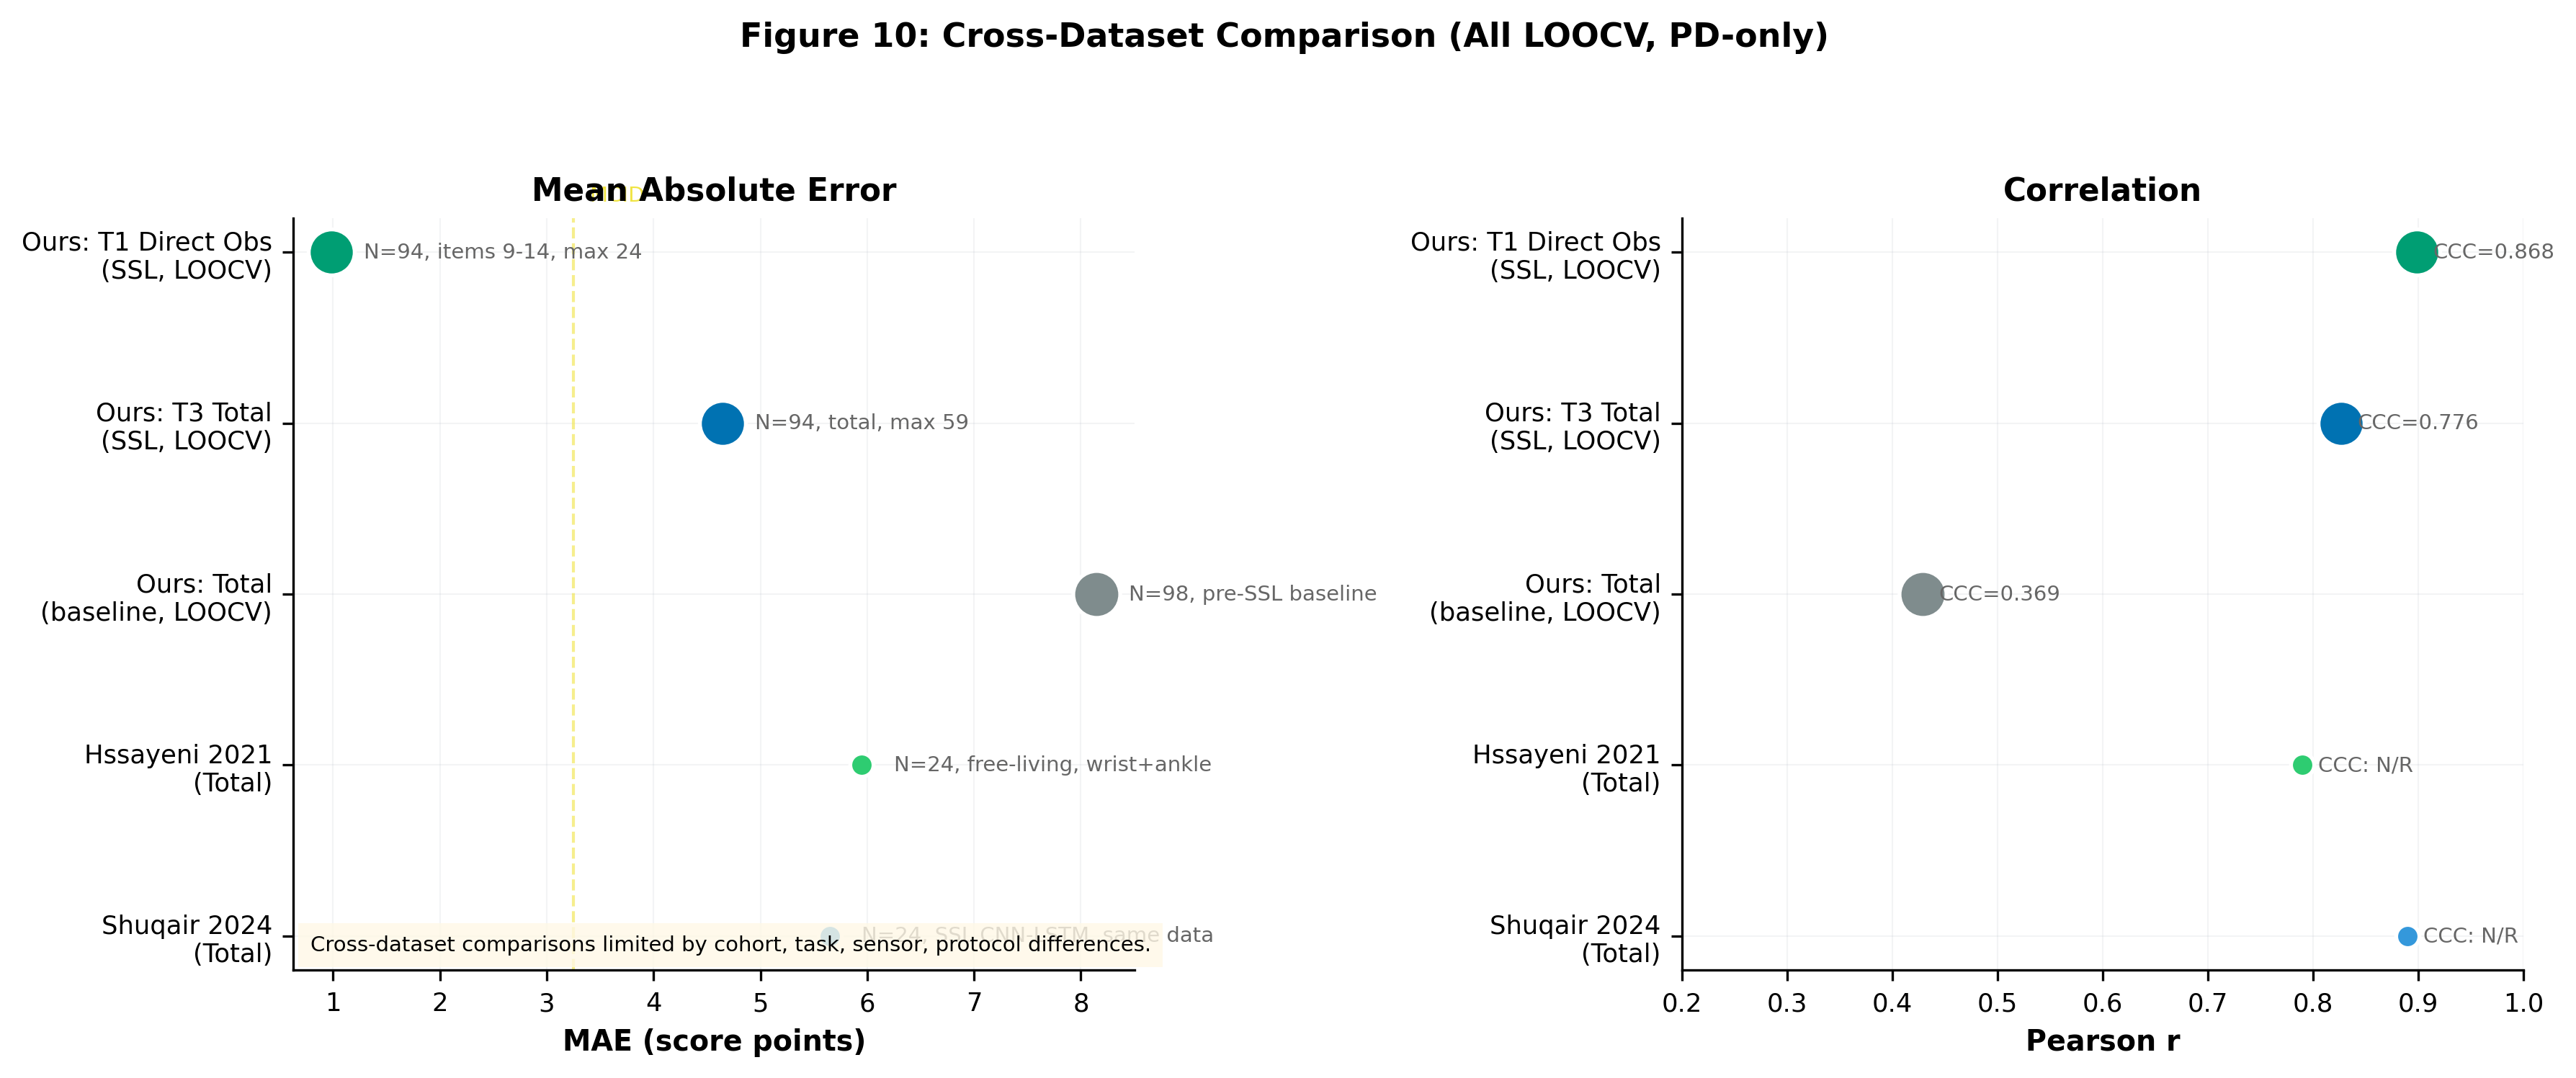
\includegraphics[width=\textwidth]{figures/fig10_cross_dataset.png}
\caption{Cross-dataset comparison (all PD-only LOOCV where available). Left: MAE; right: Pearson r with CCC annotations. Our SSL results on WearGait-PD (N=94) achieve lower MAE than prior work on smaller cohorts (N=24), but cross-dataset comparisons are limited by protocol, cohort, task, and sensor differences.}
\label{fig:cross}
\end{figure}
\begin{table}[H]
\centering
\caption{Cross-dataset comparison with published UPDRS-III regression.}
\label{tab:cross_dataset}
\small
\begin{tabular}{llllllccl}
\toprule
Study & Year & Dataset & N & Sensors & Evaluation & MAE & r & CCC \\
\midrule
\textbf{This work (T1, SSL)} & 2026 & WearGait-PD & 94 PD & 13 IMUs & PD LOOCV & 0.99* & 0.899 & 0.868 \\
\textbf{This work (T3, SSL)} & 2026 & WearGait-PD & 94 PD & 13 IMUs & PD LOOCV & 4.65 & 0.827 & 0.776 \\
This work (T3, baseline) & 2026 & WearGait-PD & 98 PD & 13 IMUs & PD LOOCV & 8.15 & 0.429 & 0.369 \\
Hssayeni et al. & 2021 & Physionet & 24 PD & wrist+ankle gyro & PD LOOCV & 5.95 & 0.79 & N/R \\
Shuqair et al. & 2024 & Same Physionet & 24 PD & wrist+ankle gyro & PD LOOCV & $\sim$5.65 & 0.89 & N/R \\
Sotirakis et al. & 2023 & Oxford & 74 PD & wrist+back & 5-fold CV\textsuperscript{\dag} & RMSE=10.02 & --- & N/R \\
\bottomrule
\end{tabular}

\smallskip
\footnotesize{*Items 3.9--3.14 subscore (max 24), not total UPDRS-III (max 132). \textsuperscript{\dag}Visit-level CV with potential within-subject leakage. N/R = not reported. Cross-dataset comparison is limited by cohort, task, sensor, and protocol differences.}
\end{table}

\subsection{Negative Results}

Negative results strengthen the ceiling argument. Seven deep learning configurations (Transformer, InceptionTime, SensorGNN; Table~\ref{tab:dl}) all produced MAE~$>$~10, consistent with overfitting at N~=~178. Additional failed approaches included: item decomposition (52\% worse), mixture-of-experts, cross-sensor coordination features, and freezing-of-gait transfer (AUC~=~0.500). Among the five anti-compression proposals, only SSL ranking produced material CCC improvement; per-item ordinal classification, pairwise contrastive boosting, SMOGN augmentation, and NGBoost distributional regression all failed (Table~\ref{tab:ssl_ablation}). This convergence of diverse approaches on a compression ceiling supports the interpretation that the barrier is representational (insufficient calibration anchors) rather than purely methodological.

\section{Discussion}

\subsection{SSL Ranking Mechanism}

The central methodological contribution is the use of healthy controls as calibration anchors for severity estimation. Pure PD-only regression (N=94) suffers from sparse support at the low-severity end of the distribution: few PD subjects have UPDRS near zero, so the model has little basis for calibrated low-end predictions and shrinks toward the cohort mean. Adding 80 HC subjects (UPDRS approximately 0--3) densifies this low end, providing the statistical anchoring that the PD-only cohort lacks. The XGBRanker (Stage 1) learns that HC subjects correspond to severity rank 0 and PD subjects to ordinal ranks 1..N$_{\text{PD}}$. This ranking task is statistically simpler than exact score prediction because it requires ordinal discrimination rather than precise score estimation. The ranker's leaf indices encode this severity ordering as a categorical embedding, which the downstream LightGBM regressor (Stage 2) uses to produce calibrated predictions. This strategy may prove useful for other clinical scale predictions with matched healthy controls, although this will require external validation.

Four mechanisms explain the improvement. First, \emph{N amplification}: pure PD-only regression has N=94; SSL uses all 178 subjects for the ranking representation. Second, \emph{HC as calibration anchors}: HC subjects (UPDRS approximately 0--3) provide dense reference points for ``definitely low severity,'' anchoring the prediction range. Third, \emph{ranking is better conditioned than regression}: ordinal discrimination requires only that the model preserve order, not absolute spacing, reducing the statistical power needed. Fourth, \emph{leaf features encode nonlinear severity partitions}: the 900 leaf indices create a severity-aware embedding that captures nonlinear interactions the original features cannot express, while regularization through the pairwise ranking objective prevents overfitting.

A potential concern is whether the SSL improvement reflects genuine within-PD calibration or merely PD-vs-HC group discrimination. Two observations argue for the former. First, the final evaluation is PD-only LOOCV---HC subjects never appear in test folds, so any CCC improvement must reflect better ordering and calibration within PD. Second, the T3 (total) improvement is the largest in absolute CCC terms (0.37 to 0.78), precisely where the baseline is most compressed; group membership alone could not explain this differential pattern across targets.

\subsection{Observable Subscore as Actionable Endpoint}

The directly observable subscore (items 3.9--3.14) achieves CCC~=~0.868 with MAE~=~0.986, well below the MCID of 3.25 points. While the MCID of 3.25 was derived for total-score longitudinal change\cite{horvath2015} and a subscore-specific MCID has not been established, the sub-MCID prediction error for the directly observable subscore suggests clinically useful single-assessment accuracy. This subscore could serve as a high-frequency secondary endpoint for interventions targeting axial motor function, including dopaminergic therapy titration for gait-related symptoms and monitoring of gait-related falls risk. Our findings suggest that modality-matched subscores merit prospective evaluation as primary endpoints rather than the total composite score.

\subsection{Observability Ceiling}

The CCC gradient---0.56 (direct) to 0.12 (partial) to 0.18 (not observable)---reflects a modality constraint, not a methodological limitation. Rigidity (item 3.3) requires passive manipulation by an examiner; speech (3.1) and facial expression (3.2) are auditory and visual assessments. These items constitute 82\% of the total score range. The convergence of 12+ distinct modeling approaches on MAE~$\approx$~8 for total UPDRS-III, combined with the observability gradient, supports this interpretation. We acknowledge that this conclusion rests on a single dataset.

\subsection{Foundation Model Paradigm}

Frozen MOMENT-1 embeddings reduced total-score MAE by 0.71 points (p~=~0.0039) in mixed evaluation. Using frozen pretrained models as feature extractors circumvents the overfitting that causes deep learning to fail at N~=~178. The FM advantage diminished in PD-only evaluation, suggesting embeddings primarily encode PD-vs-HC group features. However, FM dimensions appeared among top features for the observable subscore, indicating complementary temporal pattern capture beyond handcrafted statistics.

\subsection{Comparison with Prior Art}

Our T3 SSL result (MAE~=~4.65, N=94, LOOCV) compares favorably with Hssayeni et~al.\ (MAE~=~5.95, N=24, LOOCV) and Shuqair et~al.\ (MAE~$\sim$5.65, N=24, LOOCV) on 4x more subjects with controlled gait rather than free-living ADL. However, these comparisons are necessarily cross-dataset. Importantly, prior work reported only r and MAE; CCC was not available for comparison. We suggest that future UPDRS regression studies report CCC alongside calibration slope and MAE, since r alone ignores calibration and MAE alone ignores discrimination.

\subsection{The Compression Problem in Small-N Clinical Regression}

The compression problem is general to small-N clinical regression: when training data is limited, gradient-boosted models minimize expected loss by shrinking predictions toward the population mean. Our baseline demonstrates this concretely: T3 calibration slope = 0.104 (predictions span only 10\% of the true range), Q1 overpredicted by +14 points, Q4 underpredicted by $-$14 points. MAE~=~8.086 appears reasonable, but CCC~=~0.186 indicates poor agreement caused by severe range compression and miscalibration. SSL ranking increases slope to 0.576, partially solving this fundamental challenge.

\subsection{Limitations}

(1) Results are from a single dataset; cross-dataset validation is needed. (2) All recordings are controlled gait, not free-living. (3) Medication state was not controlled. (4) HC were older than PD (74.6 vs 66.9 years), motivating PD-only evaluation. (5) N~=~94 PD subjects limits statistical power. (6) P0 baseline uses 5-split (N=95) while P5 SSL uses LOOCV (N=94); direct comparison requires noting the protocol difference. (7) The three-level observability classification involves judgment calls for partially observable items. (8) This is cross-sectional; longitudinal change detection may differ. (9) 23 PD subjects had deep brain stimulation.

\subsection{Future Directions}

Five directions are most promising. First, longitudinal within-subject tracking using the observable subdomain. Second, cross-dataset transfer to validate the SSL ranking mechanism and observability gradient. Third, the 5-to-2 sensor reduction pathway; competitive wrist-only performance suggests smartwatch-based monitoring may be feasible. Fourth, establishing a subscore-specific MCID. Fifth, multi-site validation to assess generalizability across clinical settings.

\section{Methods}

\subsection{Dataset}

WearGait-PD\cite{weargait} (Synapse syn55052683) comprises 100 PD and 85 HC participants, of whom 178 (98 PD, 80 HC) had complete recordings. Each subject wore 13 Xsens MTw Awinda IMU sensors at: lower back, bilateral wrists, bilateral mid-lateral thighs, bilateral lateral shanks, bilateral dorsal feet, bilateral ankles, xiphoid process, and forehead. Sensors sampled at 100~Hz recording triaxial accelerometer and gyroscope data (78 total channels). Participants completed five standardized tasks: self-paced walking, hurried-pace walking, Timed Up-and-Go, balance assessment, and tandem gait, with pressure-mat variants. Motor severity was assessed using MDS-UPDRS Part III by trained clinicians.

\subsection{Preprocessing and Feature Extraction}

\textbf{Handcrafted features (1,752):} Per sensor and channel: RMS, standard deviation, range, IQR, skewness, kurtosis, jerk, zero-crossing rate; Welch PSD in locomotor (0.5--3~Hz), tremor (3--8~Hz), and high-frequency (8--25~Hz) bands with band ratios; spectral entropy; autocorrelation-based gait regularity. Additional: foot contact spatiotemporal metrics, task-contrast deltas, walkway features, and clinical covariates (age, sex, disease duration, height, weight, DBS status). Features aggregated as mean across all recordings per subject.

\textbf{Foundation model embeddings (768):} Frozen MOMENT-1-base encoder\cite{moment2024}, 768-dimensional embeddings from 26 accelerometer/gyroscope magnitude channels (13 sensors), truncated to 512 samples (5.12~s), per-channel z-normalized globally across all recordings. Output averaged per subject. Deterministic (cached to disk).

\subsection{Feature Selection}

XGBoost gain-based importance ranking (n\_estimators=300, max\_depth=4, learning\_rate=0.05, reg\_lambda=2.0, objective=reg:absoluteerror) selected top-K features within each CV fold (K=500 for CCC-optimized and SSL pipelines; K=150 for baseline held-out; K=300 for fused FM+v2).

\subsection{SSL Ranking Pipeline (P5)}

\textbf{Stage 1 (XGBRanker, N=178):} All subjects used for ranking representation. HC subjects receive rank label 0; PD subjects receive ordinal rank labels 1..N$_{\text{PD}}$ sorted by ascending target score. XGBRanker parameters: n\_estimators=300, max\_depth=4, learning\_rate=0.05, reg\_lambda=2.0, objective=rank:pairwise. Three-seed ensemble (seeds 42, 123, 456). Single query group containing all subjects.

\textbf{Stage 2 (Leaf extraction + LGB regression, PD-only):} Leaf indices extracted via ranker.apply() for each of 3 ranker seeds, producing 3 $\times$ 300 = 900 leaf features per subject. Combined with K=500 selected original features (total 1,400 features). LightGBM regression on PD-only subjects: n\_estimators=2,000, learning\_rate=0.03, max\_depth=6, num\_leaves=31, reg\_lambda=0.3, min\_data\_in\_leaf=8, colsample\_bytree=0.5, objective=mse. Five-seed ensemble (seeds 42, 123, 456, 789, 2024). Early stopping at 100 rounds on 15\% validation holdout. Predictions clipped to target range.

\subsection{Target Definitions}

T1 (direct observable): sum of items 9--14 (each 0--4, range 0--24). T2 (broad observable): sum of items 7--14, where items 7 and 8 scored as max(right, left) (range 0--32). T3 (total UPDRS-III): sum of all 18 items (empirical range 0--59 in this cohort).

\subsection{Evaluation Protocol}

\emph{PD-only LOOCV} (N=94): leave-one-PD-subject-out with feature selection re-run per fold. Used for P5 SSL validation and baseline observability decomposition. \emph{PD-only 5-split CV} (N=95): stratified by target quartiles. Used for P0--P4 compression ablation. \emph{PD-only 10-split CV} (N=98): stratified by UPDRS bins, seeds 1--10. Used for FM ablation and sensor ablation. The different protocols are explicitly labeled in all tables and figures.

\subsection{Three-Level Observability Classification}

\emph{Directly observable} (items 3.9--3.14): arising, gait, freezing, postural stability, posture, body bradykinesia---motor signs directly expressed during ambulation. \emph{Partially observable} (3.5--3.8, 3.15--3.17): hand movements, pronation-supination, toe tapping, leg agility, postural/kinetic/rest tremor---limb items indirectly reflected in gait. \emph{Not observable} (3.1--3.4, 3.18): speech, facial expression, rigidity (neck + extremities), finger tapping, tremor constancy. Direct + partial + unobservable = total (reconstruction error = 0.0).

\subsection{Statistical Analysis}

Primary metric: Lin's CCC\cite{lin1989}. BCa bootstrap CIs (N=10,000, stratified by group). Model comparisons: paired bootstrap for LOOCV, Wilcoxon signed-rank for multi-split. Multiple comparison correction: Holm-Bonferroni. Effect sizes: Cohen's d. MCID: 3.25 points for improvement, 4.63 for worsening (Horvath 2015)\cite{horvath2015}, applied as contextual benchmark. Bland-Altman for systematic bias. Partial correlation controlling for age and disease duration.
\begin{table}[H]
\centering
\caption{Hyperparameter specification for all pipelines.}
\label{tab:hyperparams}
\begin{tabular}{llll}
\toprule
Parameter & Baseline LGB & CCC-Optimized LGB & XGBRanker (Stage 1) \\
\midrule
n\_estimators & 2,000 & 2,000 & 300 \\
learning\_rate & 0.03 & 0.03 & 0.05 \\
max\_depth & 6 & 6 & 4 \\
num\_leaves & 31 & 31 & --- \\
reg\_lambda & 3.0 & 0.3 & 2.0 \\
min\_data\_in\_leaf & 20 & 8 & --- \\
colsample\_bytree & 1.0 & 0.5 & --- \\
objective & mae & mse & rank:pairwise \\
early\_stopping & 100 & 100 & --- \\
val\_frac & 0.15 & 0.15 & --- \\
Feature K & 150 & 500 & 500 \\
Seeds & [42,123,456,789,2024] & [42,123,456,789,2024] & [42,123,456] \\
\bottomrule
\end{tabular}

\smallskip
\footnotesize{Feature selection uses XGBoost (n\_estimators=300, max\_depth=4, lr=0.05, reg\_lambda=2.0, objective=reg:absoluteerror) inside each CV fold. CCC-optimized parameters identified via autoresearch (67 configurations tested).}
\end{table}

\subsection{Code and Data Availability}

WearGait-PD is available on Synapse (syn55052683)\cite{weargait}. Analysis code will be available at [repository URL].

\section*{References}
\begin{thebibliography}{99}
\bibitem{gbd2019} GBD 2019 Collaborators. Global, regional, and national burden of neurological disorders, 1990--2019. \emph{Lancet Neurol.} 20, 797--820 (2021).
\bibitem{horvath2015} Horvath, K. et al. Minimal clinically important difference on the Motor Examination part of MDS-UPDRS. \emph{Parkinsonism Relat.\ Disord.} 21, 1421--1426 (2015).
\bibitem{hssayeni2021} Hssayeni, M. D. et al. Wearable sensors for estimation of Parkinsonian tremor severity during free body movement. \emph{BioMed.\ Eng.\ OnLine} 20, 24 (2021).
\bibitem{shuqair2024} Shuqair, H. et al. Self-supervised representation learning for motor severity estimation. \emph{Bioengineering} 11, 689 (2024).
\bibitem{sotirakis2023} Sotirakis, C. et al. Identification of motor progression in Parkinson's disease using wearable sensors. \emph{npj Parkinsons Dis.} 9, 74 (2023).
\bibitem{he2024} He, S. et al. Predicting levodopa response using wearable sensors. \emph{J.\ NeuroEng.\ Rehab.} 21, 47 (2024).
\bibitem{trip2025} Li, J. et al. TRIP: Transformer-based IMU pretraining for Parkinson's disease. \emph{arXiv} 2510.15748 (2025).
\bibitem{lin1989} Lin, L. I.-K. A concordance correlation coefficient to evaluate reproducibility. \emph{Biometrics} 45, 255--268 (1989).
\bibitem{weargait} WearGait-PD dataset. \emph{Sci.\ Data} (2026). doi:10.1038/s41597-026-06806-2.
\bibitem{moment2024} Goswami, M. et al. MOMENT: A family of open time-series foundation models. \emph{ICML} (2024).
\bibitem{lightgbm} Ke, G. et al. LightGBM: A highly efficient gradient boosting decision tree. \emph{NeurIPS} (2017).
\bibitem{xgboost} Chen, T. \& Guestrin, C. XGBoost: A scalable tree boosting system. \emph{KDD} (2016).
\bibitem{goetz2008} Goetz, C. G. et al. Movement Disorder Society-sponsored revision of the Unified Parkinson's Disease Rating Scale (MDS-UPDRS). \emph{Mov.\ Disord.} 23, 2129--2170 (2008).
\end{thebibliography}

\appendix

\section{The Machine Learning Pipeline}

This section provides a self-contained explanation of the machine learning methodology for clinical readers.

\subsection{Gradient-Boosted Decision Trees}

Gradient-boosted decision trees (GBDT) build an ensemble of simple decision trees sequentially (Figure~\ref{fig:gbdt}). Each tree corrects the residual errors of the previous ensemble. LightGBM and XGBoost are two efficient implementations. A single tree partitions the feature space into leaf nodes, each predicting a constant value. The ensemble of 2,000 trees produces a prediction by summing all tree outputs. Early stopping monitors validation error and halts training when no improvement occurs for 100 consecutive rounds, preventing overfitting.
\begin{figure}[H]
\centering
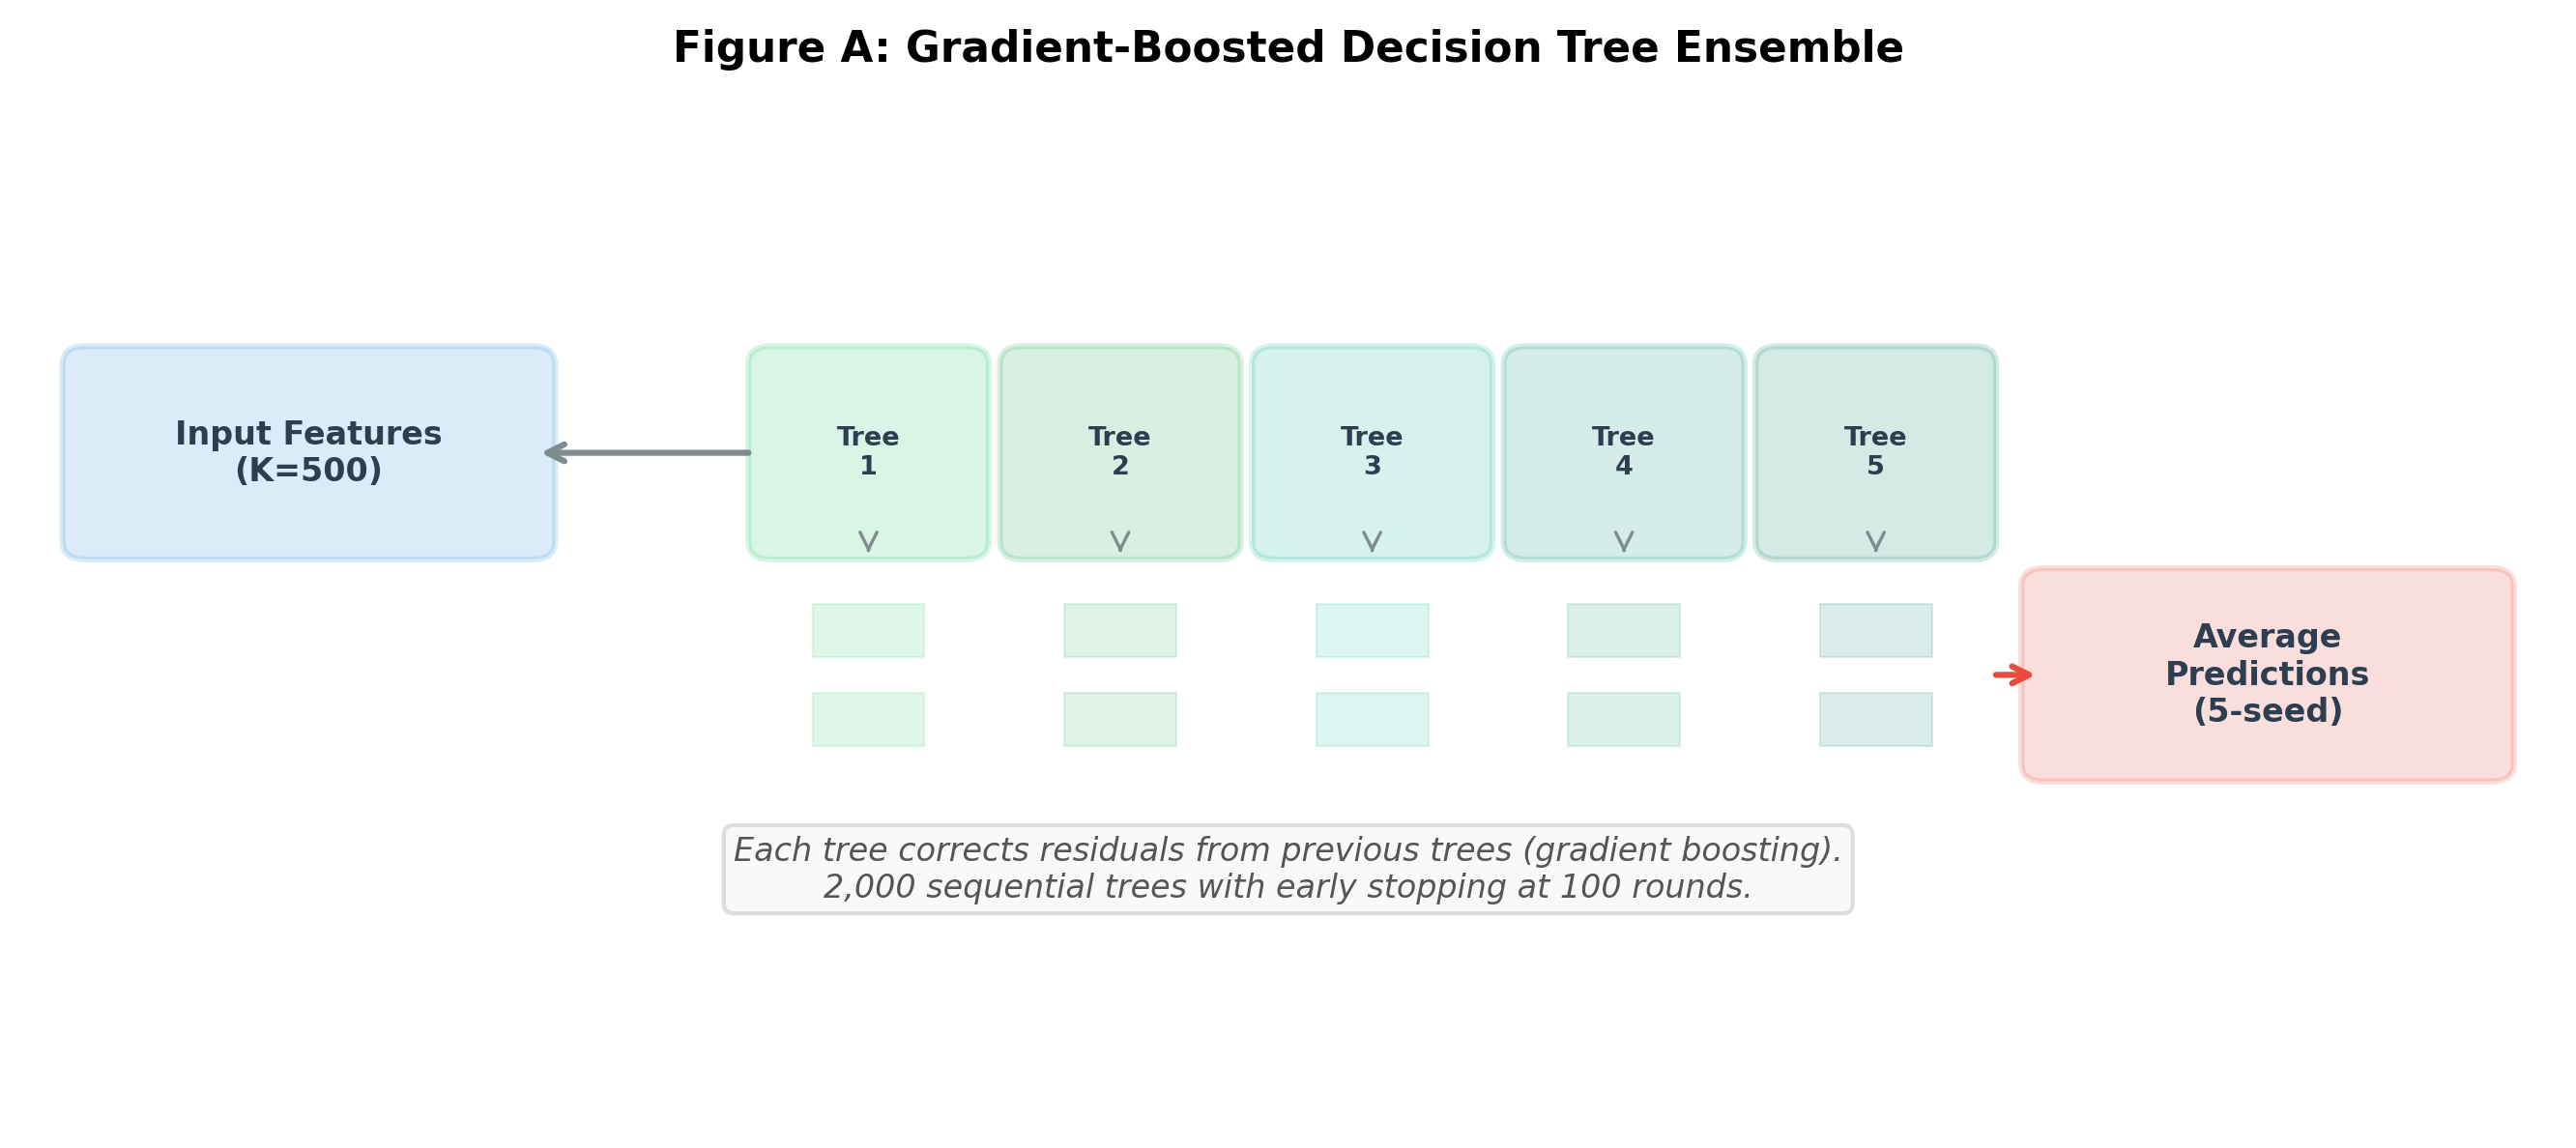
\includegraphics[width=\textwidth]{figures/figA_gbdt.png}
\caption{Gradient-boosted decision tree ensemble. Each tree corrects residuals from previous trees. Final prediction is the sum of all 2,000 tree outputs. Early stopping at 100 rounds prevents overfitting.}
\label{fig:gbdt}
\end{figure}

\subsection{MSE vs MAE Loss}

The choice of loss function affects how the model treats errors of different magnitudes (Figure~\ref{fig:mse_mae}). MAE (mean absolute error) loss treats all errors equally: a 1-point error and a 10-point error contribute proportionally. MSE (mean squared error) loss penalizes large errors quadratically: a 10-point error contributes 100x more than a 1-point error. For UPDRS prediction, MSE proved superior (MAE improvement from 8.67 to 8.36) because it forces the model to reduce the most severe errors, which correspond to high-severity patients that baseline models systematically underpredict.
\begin{figure}[H]
\centering
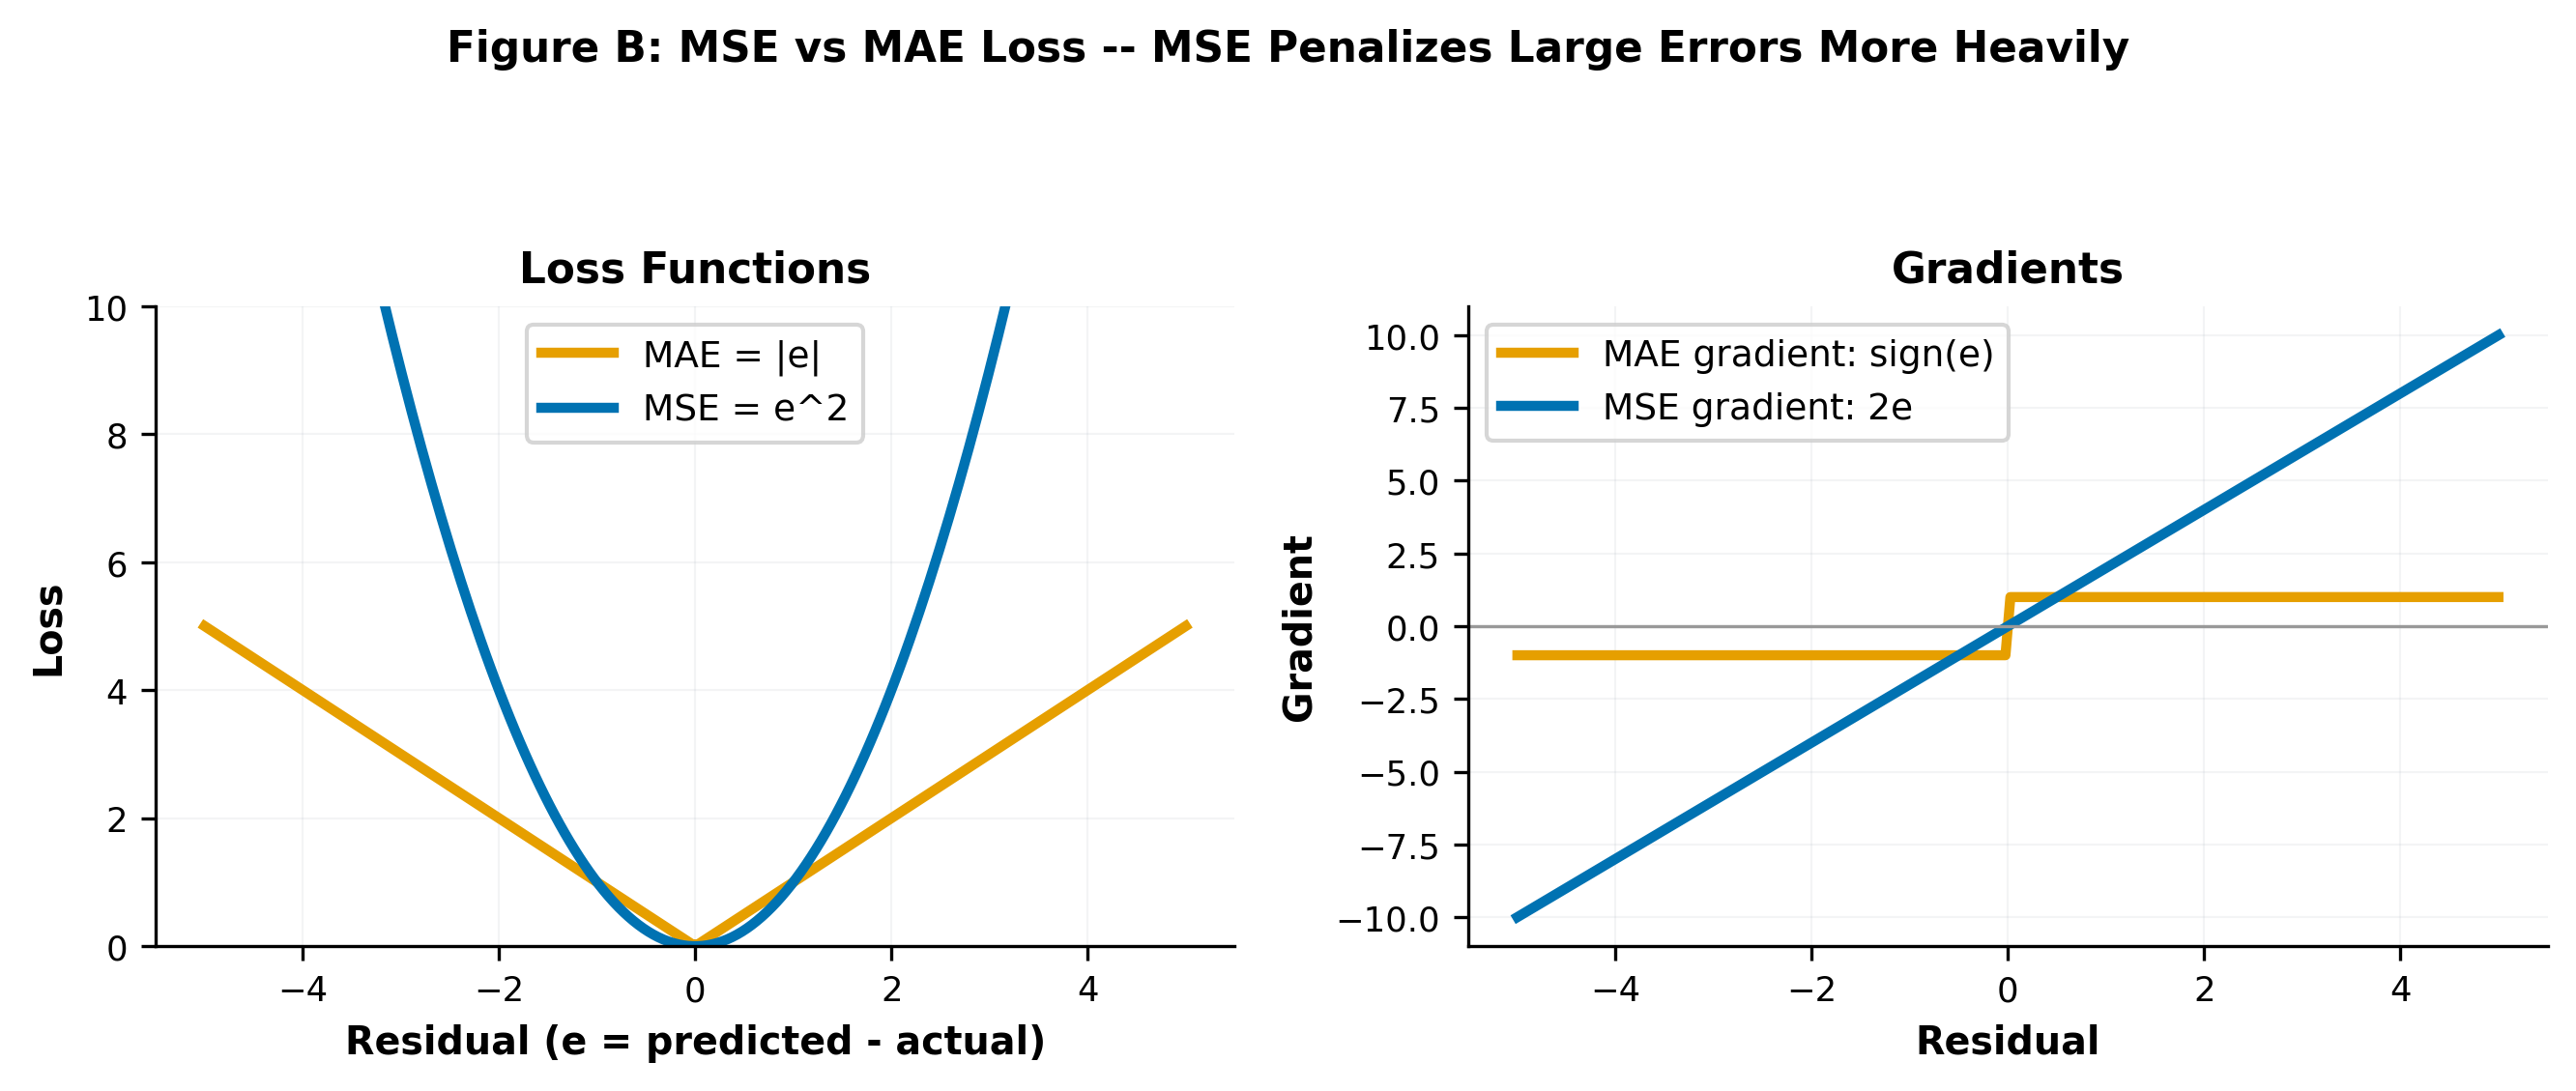
\includegraphics[width=\textwidth]{figures/figB_mse_mae.png}
\caption{MSE vs MAE loss functions and their gradients. MSE penalizes large errors more heavily, forcing the model to attend to extreme cases.}
\label{fig:mse_mae}
\end{figure}

\subsection{Feature Selection}

With 2,520 candidate features and only $\sim$95 training subjects, feature selection is critical to prevent overfitting (Figure~\ref{fig:feat_sel}). We use XGBoost importance: an XGBoost model is trained to predict the target, and features are ranked by their total gain (improvement in the loss function when the feature is used for splitting). The top K features are retained. K=500 was optimal for the CCC-optimized pipeline; K=150 sufficed for the MAE-optimized baseline. Selection is performed inside each cross-validation fold to prevent data leakage.
\begin{figure}[H]
\centering
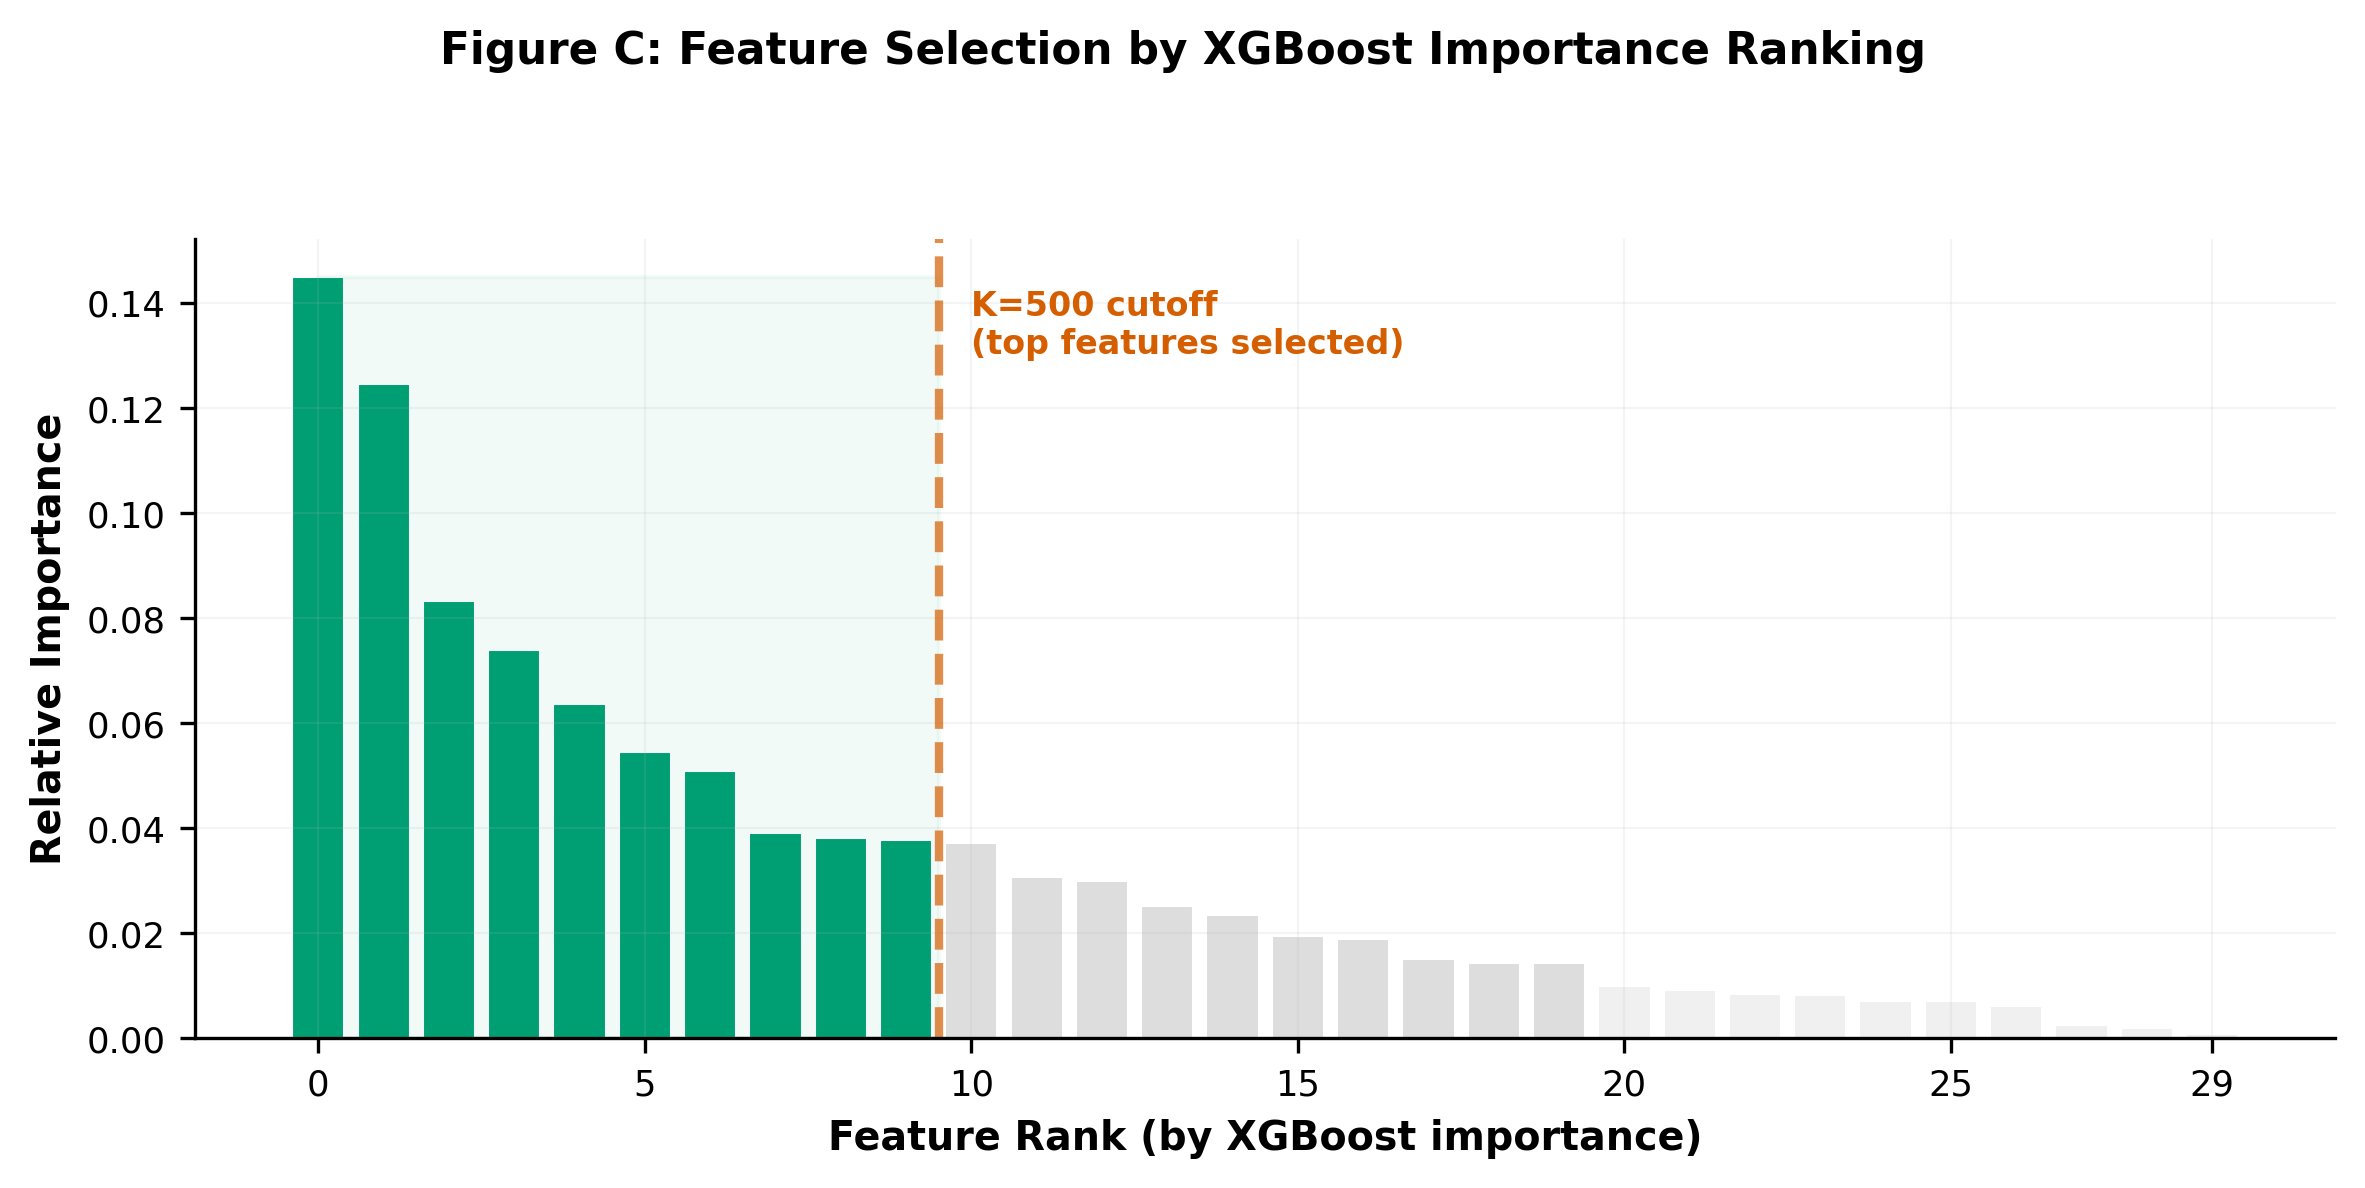
\includegraphics[width=\textwidth]{figures/figC_feature_selection.png}
\caption{Feature selection by XGBoost importance. Features ranked by total gain; top-K retained (green). The cutoff balances signal retention against overfitting risk.}
\label{fig:feat_sel}
\end{figure}

\subsection{Multi-Seed Ensemble}

Individual model predictions vary with the random seed (which affects data shuffling, feature subsampling, and validation splits). Averaging predictions across 5 independent seeds (42, 123, 456, 789, 2024) reduces this variance (Figure~\ref{fig:multi_seed}). The ensemble prediction is always at least as good as the average individual prediction, and typically better.
\begin{figure}[H]
\centering
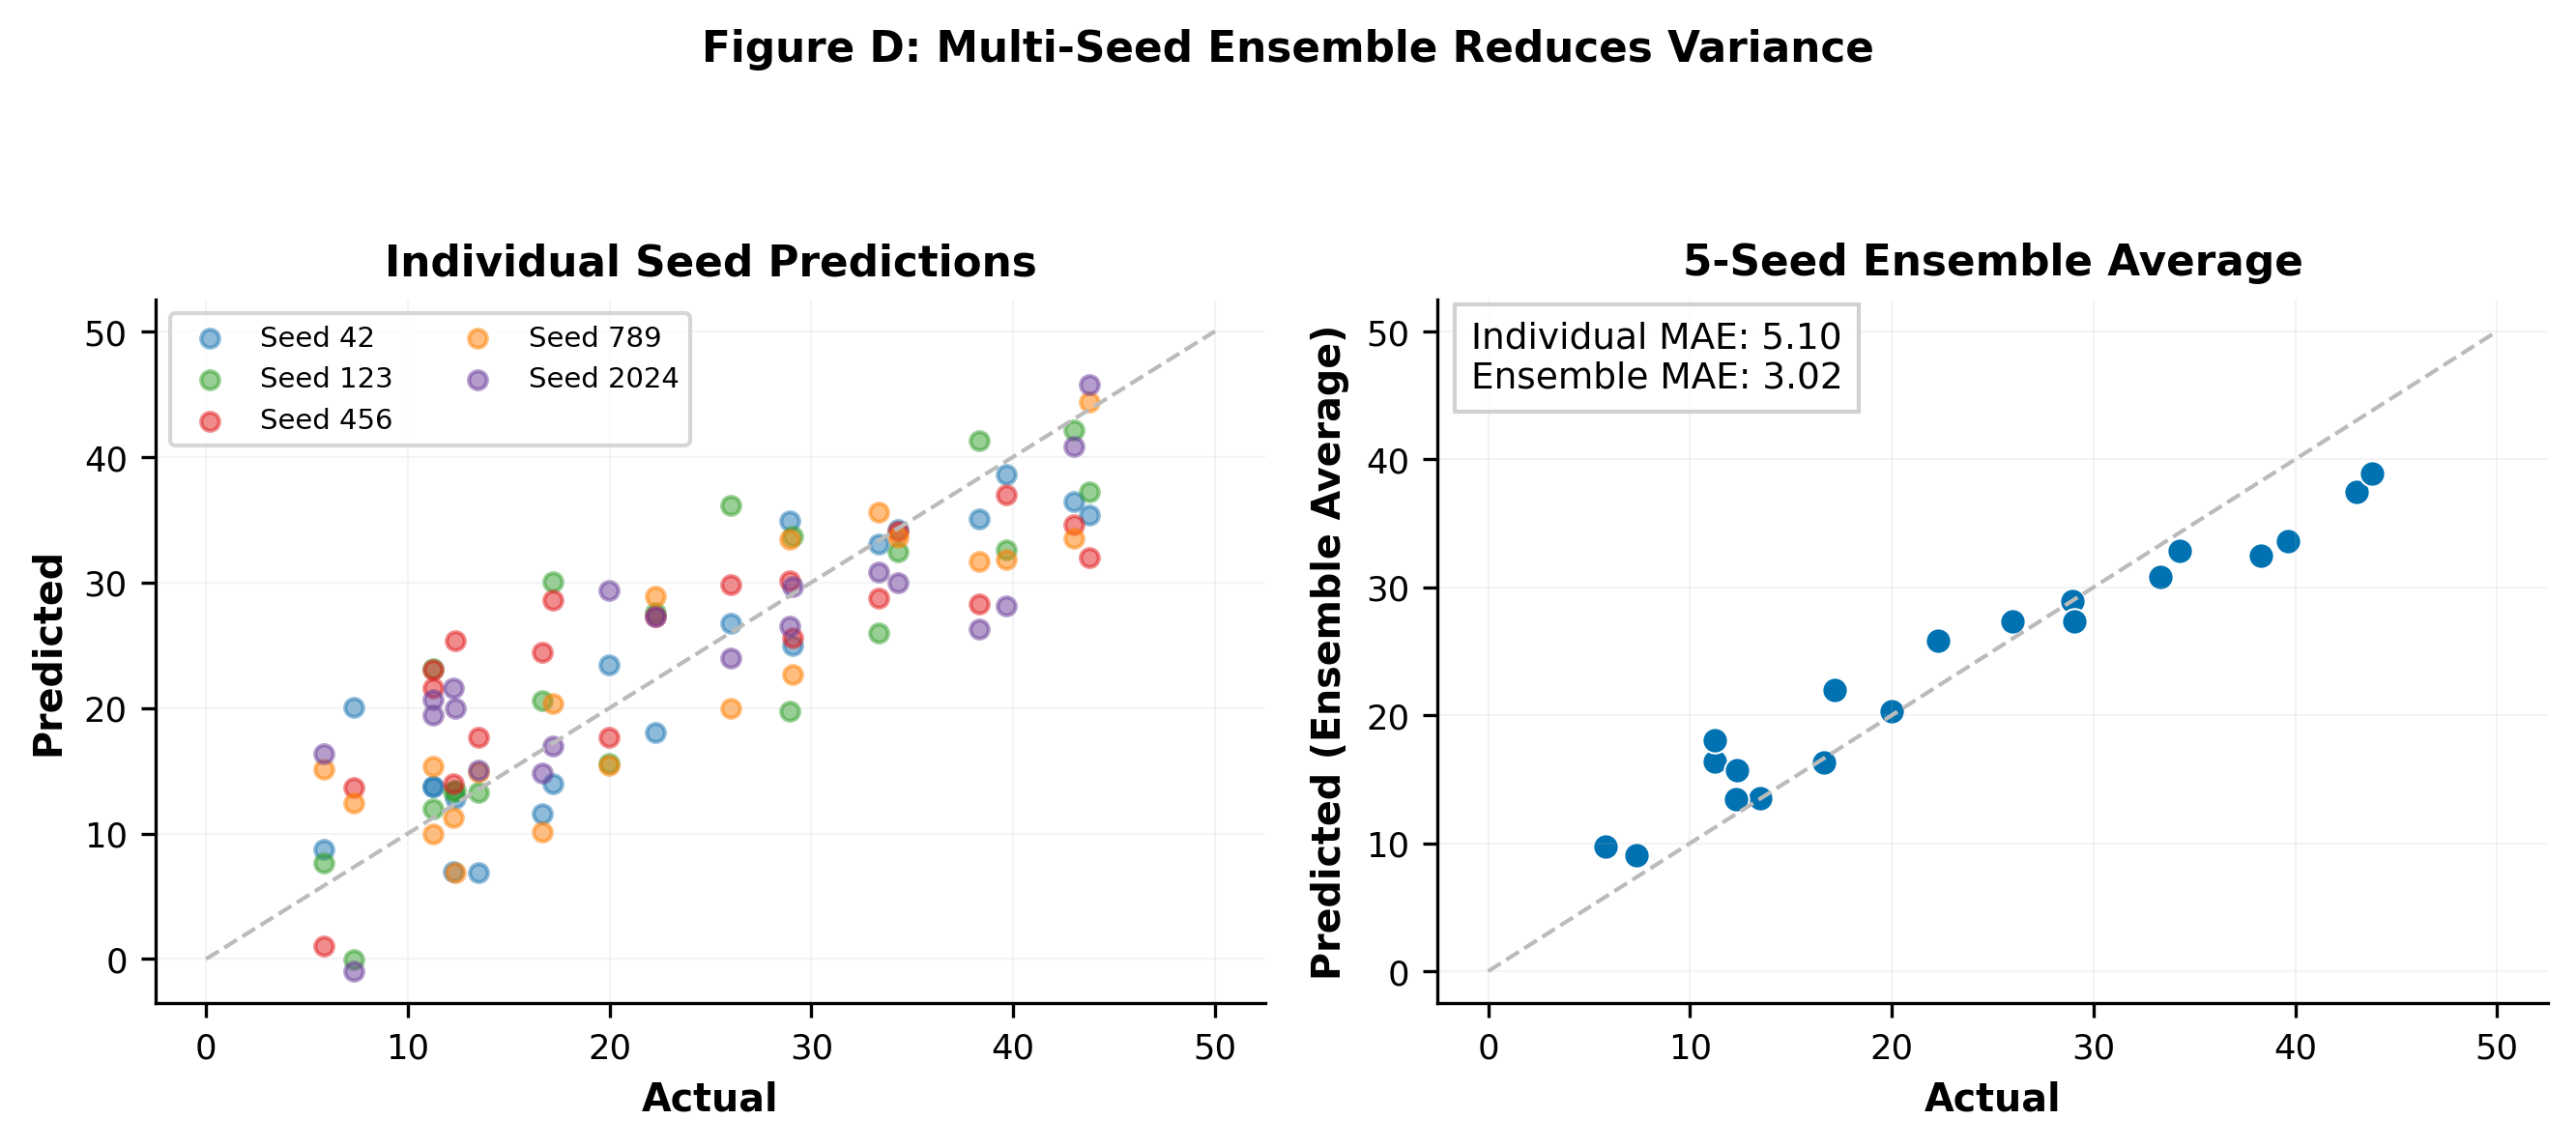
\includegraphics[width=\textwidth]{figures/figD_multi_seed.png}
\caption{Multi-seed ensemble averaging. Left: individual seed predictions show scatter. Right: 5-seed ensemble average is smoother and more accurate.}
\label{fig:multi_seed}
\end{figure}

\subsection{Foundation Model Embedding Extraction}

MOMENT-1-base is a time-series foundation model pretrained on 385 public datasets\cite{moment2024}. We use it as a frozen feature extractor (Figure~\ref{fig:fm_embed}): raw IMU signals are truncated to 512 samples (5.12s), globally z-normalized, and passed through the frozen encoder. The resulting 768-dimensional embedding captures temporal patterns learned from diverse domains, supplementing handcrafted statistical features. No gradient computation or fine-tuning is performed, ensuring deterministic outputs.
\begin{figure}[H]
\centering
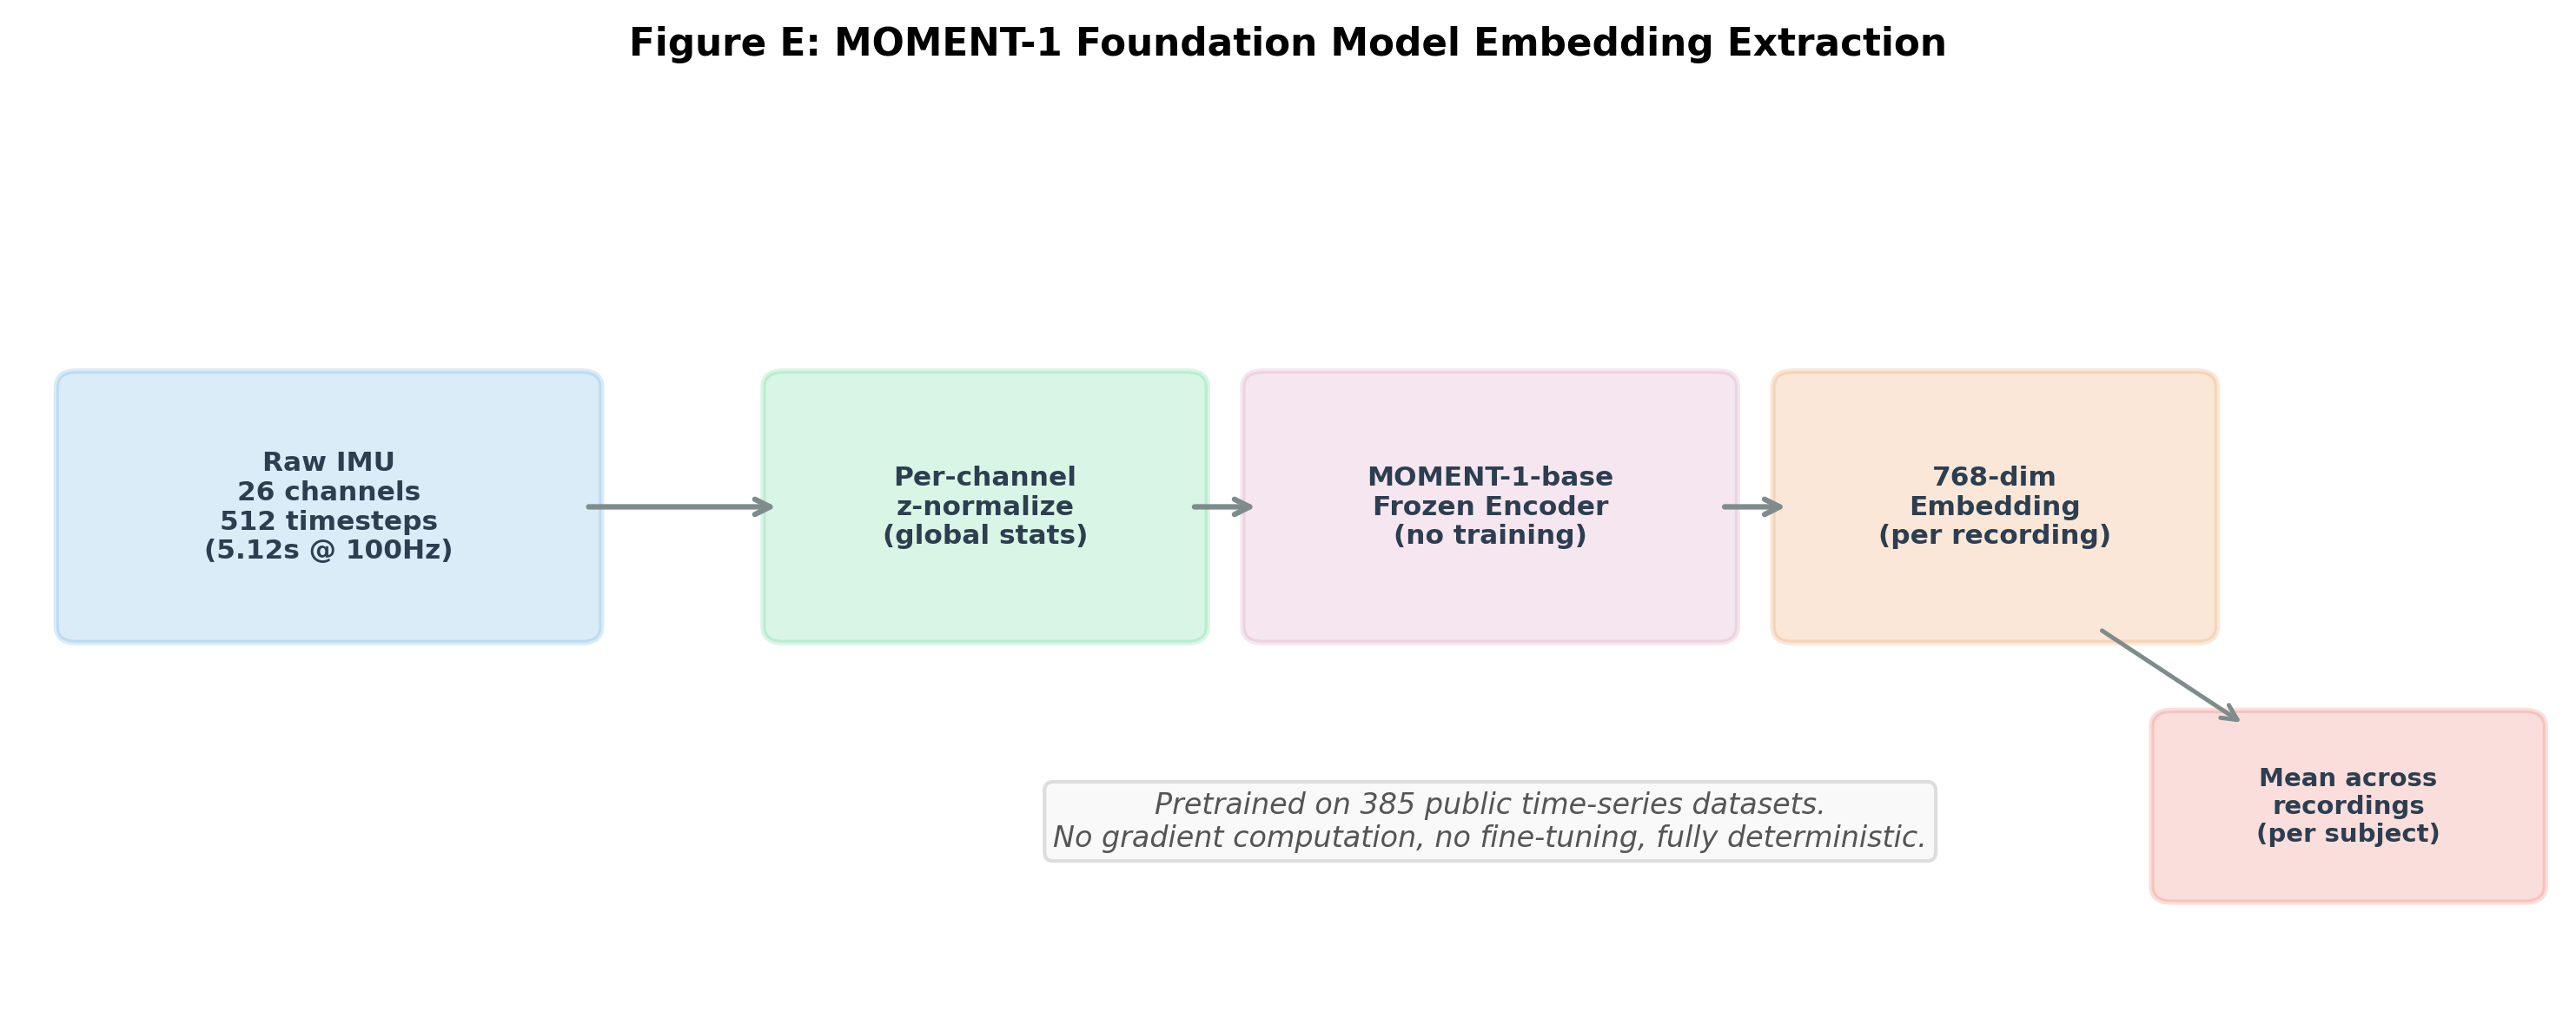
\includegraphics[width=\textwidth]{figures/figE_fm_embedding.png}
\caption{MOMENT-1 foundation model embedding extraction. Raw IMU signals are normalized and passed through the frozen encoder to produce 768-dimensional embeddings, averaged across recordings per subject.}
\label{fig:fm_embed}
\end{figure}

\subsection{Hyperparameter Choices}

Key hyperparameter differences between the baseline and CCC-optimized pipelines (Figure~\ref{fig:hp}): regularization (reg\_lambda: 3.0 to 0.3) was reduced to allow wider prediction range; min\_data\_in\_leaf (20 to 8) was the dominant knob for CCC improvement (+0.105); colsample\_bytree (1.0 to 0.5) introduced column subsampling for diversity; and objective (MAE to MSE) increased penalty on large errors. These changes collectively increased calibration slope from 0.40 to 0.69 on the observable subscore.
\begin{figure}[H]
\centering
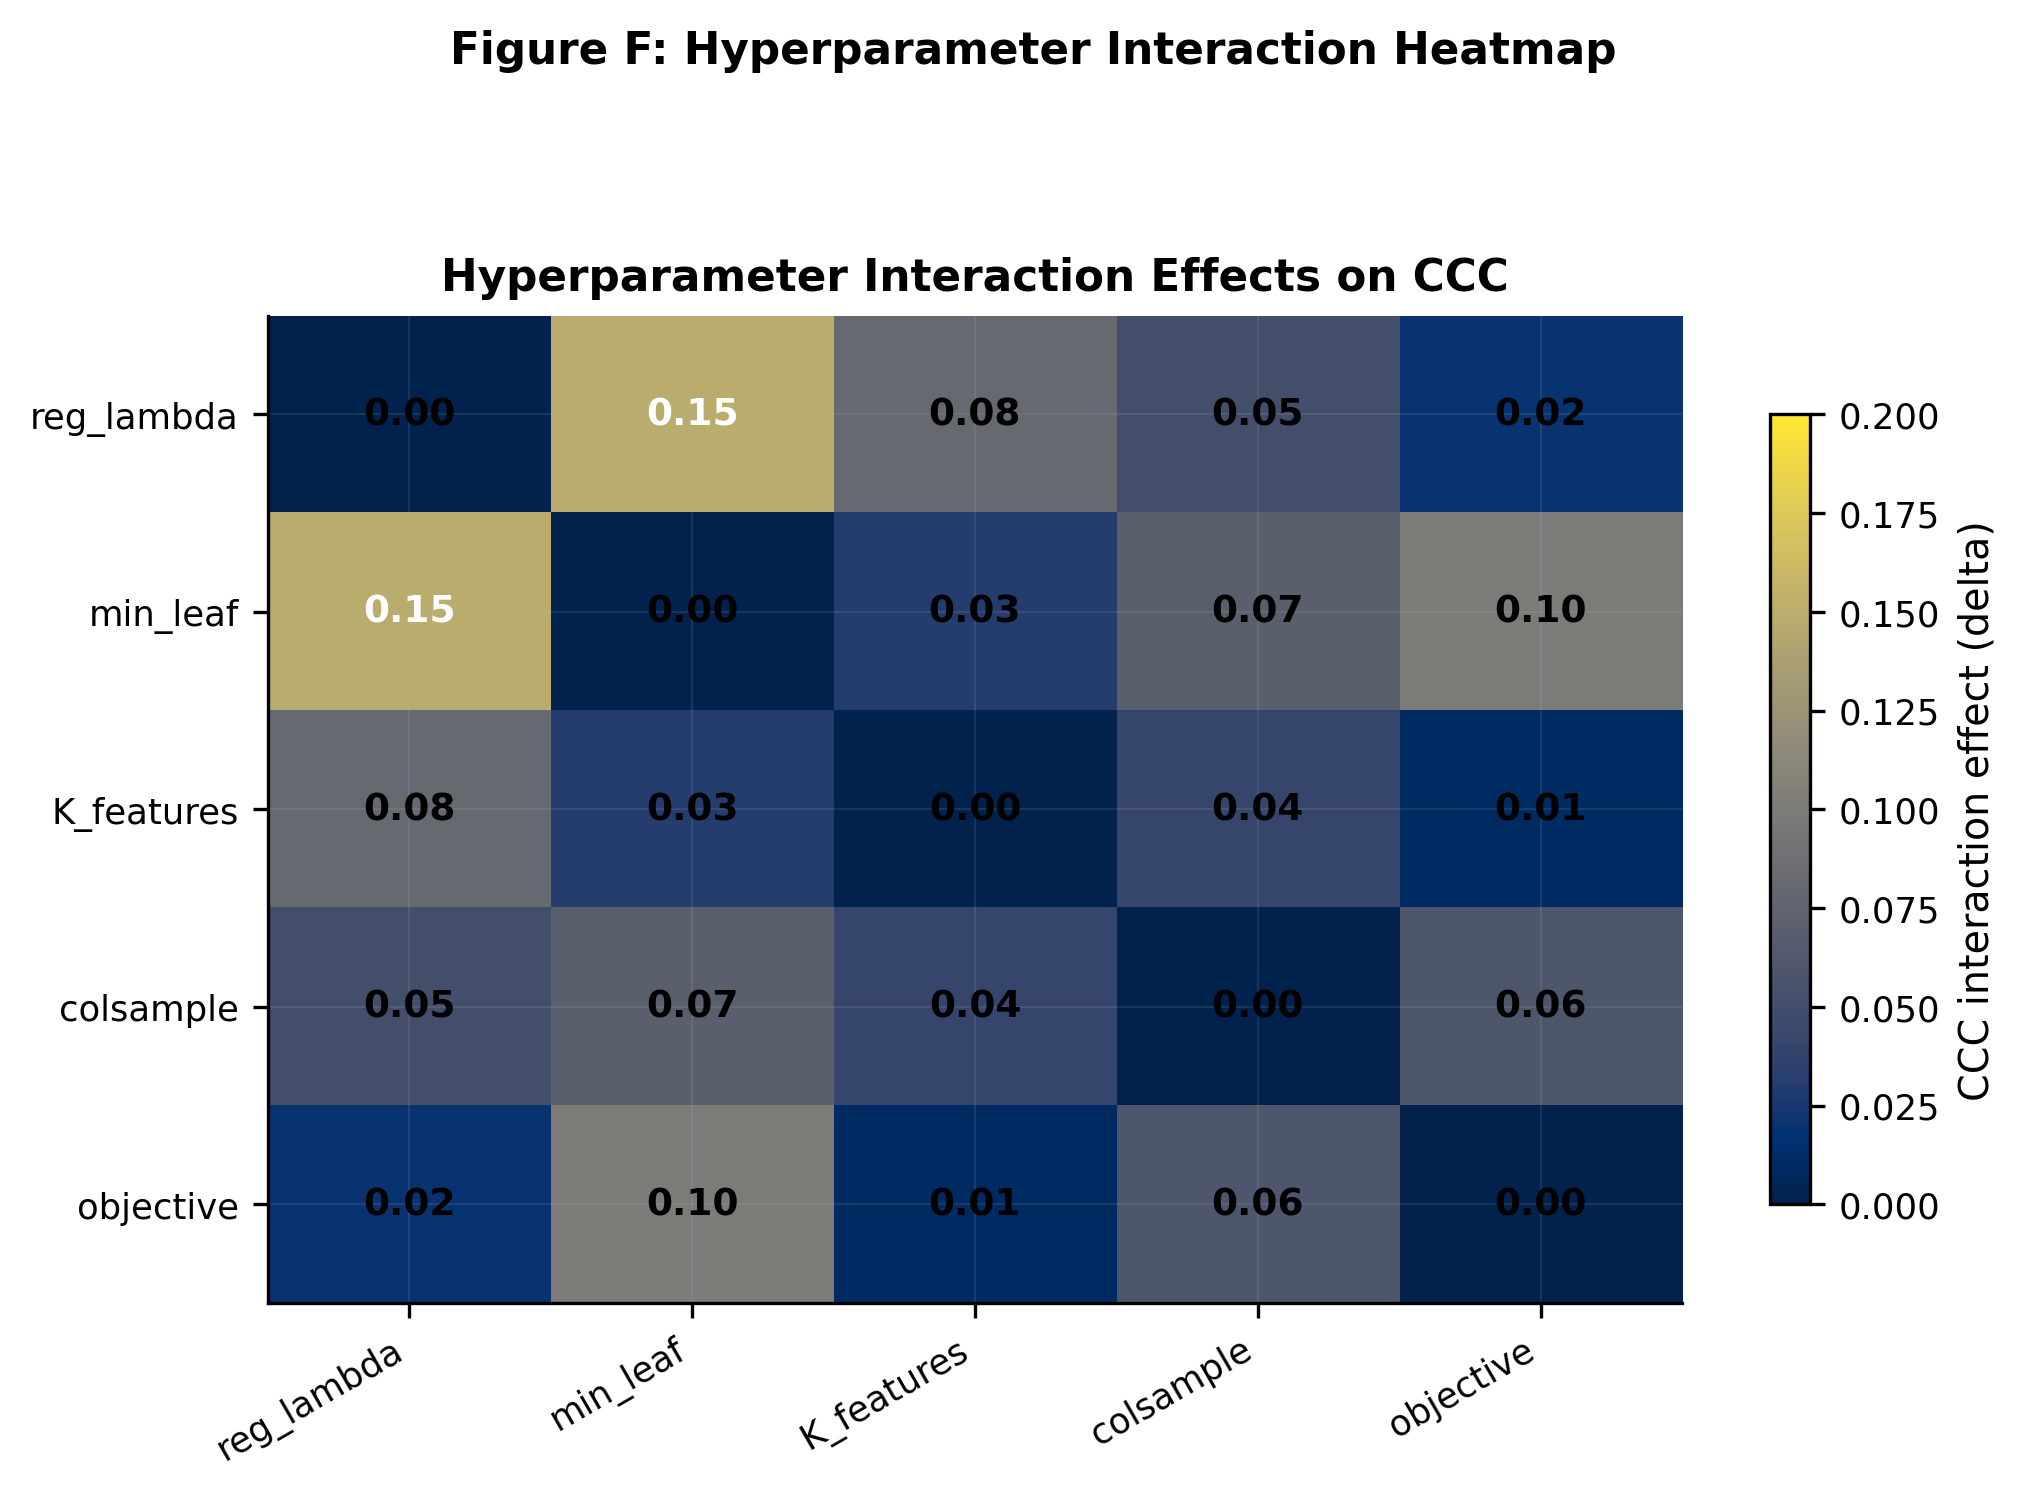
\includegraphics[width=\textwidth]{figures/figF_hp_heatmap.png}
\caption{Hyperparameter interaction effects on CCC. The strongest interaction is between reg\_lambda and min\_data\_in\_leaf, reflecting the trade-off between regularization and leaf granularity.}
\label{fig:hp}
\end{figure}

\section*{Supplementary Information}
\begin{table}[H]
\centering
\caption{Deep learning architectures (all MAE $>$ 10 on held-out test, seed=42 split).}
\label{tab:dl}
\begin{tabular}{lccc}
\toprule
Architecture & Mean MAE $\pm$ SD & Ensemble MAE & Ensemble r \\
\midrule
P1A: MAE→Transformer 128d/4L + MIL & 11.88 $\pm$ 2.70 & 10.85 & 0.590 \\
P1B: Contrastive→Transformer 128d/4L + MIL & 12.96 $\pm$ 2.22 & 11.70 & 0.349 \\
P1C: Transformer 128d/4L + MIL (scratch) & 11.96 $\pm$ 2.54 & 10.99 & 0.521 \\
P3A: InceptionTime 3blk + MIL & 13.22 $\pm$ 1.87 & 11.87 & 0.470 \\
P3B: InceptionTime 3blk + ordinal & 11.93 $\pm$ 0.93 & 10.46 & 0.436 \\
P3C: InceptionTime 3blk h24 + MIL & 12.84 $\pm$ 0.94 & 12.01 & 0.443 \\
P6A: SensorGNN 64d + MIL & 13.80 $\pm$ 0.61 & 13.68 & 0.454 \\
\bottomrule
\end{tabular}

\smallskip
\footnotesize{All DL models trained end-to-end on raw IMU windows (10s, 50\% overlap). N=178 insufficient for end-to-end deep learning. Held-out test N=36.}
\end{table}
\begin{table}[H]
\centering
\caption{Holm-Bonferroni corrected p-values across primary statistical tests.}
\label{tab:holm}
\begin{tabular}{lccc}
\toprule
Test & p (raw) & p (adjusted) & Sig. \\
\midrule
P1\_fm\_vs\_v2\_median & 0.4692 & 0.9384 & ns \\
P1\_fm\_vs\_demo\_median & 0.2991 & 0.8973 & ns \\
P2\_permutation & 0.0003 & 0.0021 & ** \\
P2\_fm\_vs\_demo\_bootstrap & 0.5924 & 0.9384 & ns \\
P2\_partial\_corr & 0.0003 & 0.0021 & ** \\
P3\_ordering\_test & 0.1721 & 0.6884 & ns \\
P4\_spearman & 0.0001 & 0.0008 & *** \\
P4\_partial\_corr & 0.0003 & 0.0021 & ** \\
\bottomrule
\end{tabular}

\smallskip
\footnotesize{Three tests survive correction: permutation (FM $>$ mean), Spearman severity ranking, and partial correlation (IMU signal beyond demographics).}
\end{table}

\end{document}
